\PassOptionsToPackage{unicode=true}{hyperref} % options for packages loaded elsewhere
\PassOptionsToPackage{hyphens}{url}
%
\documentclass[
]{book}
\usepackage{lmodern}
\usepackage{amssymb,amsmath}
\usepackage{ifxetex,ifluatex}
\ifnum 0\ifxetex 1\fi\ifluatex 1\fi=0 % if pdftex
  \usepackage[T1]{fontenc}
  \usepackage[utf8]{inputenc}
  \usepackage{textcomp} % provides euro and other symbols
\else % if luatex or xelatex
  \usepackage{unicode-math}
  \defaultfontfeatures{Scale=MatchLowercase}
  \defaultfontfeatures[\rmfamily]{Ligatures=TeX,Scale=1}
\fi
% use upquote if available, for straight quotes in verbatim environments
\IfFileExists{upquote.sty}{\usepackage{upquote}}{}
\IfFileExists{microtype.sty}{% use microtype if available
  \usepackage[]{microtype}
  \UseMicrotypeSet[protrusion]{basicmath} % disable protrusion for tt fonts
}{}
\makeatletter
\@ifundefined{KOMAClassName}{% if non-KOMA class
  \IfFileExists{parskip.sty}{%
    \usepackage{parskip}
  }{% else
    \setlength{\parindent}{0pt}
    \setlength{\parskip}{6pt plus 2pt minus 1pt}}
}{% if KOMA class
  \KOMAoptions{parskip=half}}
\makeatother
\usepackage{xcolor}
\IfFileExists{xurl.sty}{\usepackage{xurl}}{} % add URL line breaks if available
\IfFileExists{bookmark.sty}{\usepackage{bookmark}}{\usepackage{hyperref}}
\hypersetup{
  pdftitle={R @ R(D)SVS},
  pdfauthor={Jill R D MacKay},
  pdfborder={0 0 0},
  breaklinks=true}
\urlstyle{same}  % don't use monospace font for urls
\usepackage{color}
\usepackage{fancyvrb}
\newcommand{\VerbBar}{|}
\newcommand{\VERB}{\Verb[commandchars=\\\{\}]}
\DefineVerbatimEnvironment{Highlighting}{Verbatim}{commandchars=\\\{\}}
% Add ',fontsize=\small' for more characters per line
\usepackage{framed}
\definecolor{shadecolor}{RGB}{248,248,248}
\newenvironment{Shaded}{\begin{snugshade}}{\end{snugshade}}
\newcommand{\AlertTok}[1]{\textcolor[rgb]{0.94,0.16,0.16}{#1}}
\newcommand{\AnnotationTok}[1]{\textcolor[rgb]{0.56,0.35,0.01}{\textbf{\textit{#1}}}}
\newcommand{\AttributeTok}[1]{\textcolor[rgb]{0.77,0.63,0.00}{#1}}
\newcommand{\BaseNTok}[1]{\textcolor[rgb]{0.00,0.00,0.81}{#1}}
\newcommand{\BuiltInTok}[1]{#1}
\newcommand{\CharTok}[1]{\textcolor[rgb]{0.31,0.60,0.02}{#1}}
\newcommand{\CommentTok}[1]{\textcolor[rgb]{0.56,0.35,0.01}{\textit{#1}}}
\newcommand{\CommentVarTok}[1]{\textcolor[rgb]{0.56,0.35,0.01}{\textbf{\textit{#1}}}}
\newcommand{\ConstantTok}[1]{\textcolor[rgb]{0.00,0.00,0.00}{#1}}
\newcommand{\ControlFlowTok}[1]{\textcolor[rgb]{0.13,0.29,0.53}{\textbf{#1}}}
\newcommand{\DataTypeTok}[1]{\textcolor[rgb]{0.13,0.29,0.53}{#1}}
\newcommand{\DecValTok}[1]{\textcolor[rgb]{0.00,0.00,0.81}{#1}}
\newcommand{\DocumentationTok}[1]{\textcolor[rgb]{0.56,0.35,0.01}{\textbf{\textit{#1}}}}
\newcommand{\ErrorTok}[1]{\textcolor[rgb]{0.64,0.00,0.00}{\textbf{#1}}}
\newcommand{\ExtensionTok}[1]{#1}
\newcommand{\FloatTok}[1]{\textcolor[rgb]{0.00,0.00,0.81}{#1}}
\newcommand{\FunctionTok}[1]{\textcolor[rgb]{0.00,0.00,0.00}{#1}}
\newcommand{\ImportTok}[1]{#1}
\newcommand{\InformationTok}[1]{\textcolor[rgb]{0.56,0.35,0.01}{\textbf{\textit{#1}}}}
\newcommand{\KeywordTok}[1]{\textcolor[rgb]{0.13,0.29,0.53}{\textbf{#1}}}
\newcommand{\NormalTok}[1]{#1}
\newcommand{\OperatorTok}[1]{\textcolor[rgb]{0.81,0.36,0.00}{\textbf{#1}}}
\newcommand{\OtherTok}[1]{\textcolor[rgb]{0.56,0.35,0.01}{#1}}
\newcommand{\PreprocessorTok}[1]{\textcolor[rgb]{0.56,0.35,0.01}{\textit{#1}}}
\newcommand{\RegionMarkerTok}[1]{#1}
\newcommand{\SpecialCharTok}[1]{\textcolor[rgb]{0.00,0.00,0.00}{#1}}
\newcommand{\SpecialStringTok}[1]{\textcolor[rgb]{0.31,0.60,0.02}{#1}}
\newcommand{\StringTok}[1]{\textcolor[rgb]{0.31,0.60,0.02}{#1}}
\newcommand{\VariableTok}[1]{\textcolor[rgb]{0.00,0.00,0.00}{#1}}
\newcommand{\VerbatimStringTok}[1]{\textcolor[rgb]{0.31,0.60,0.02}{#1}}
\newcommand{\WarningTok}[1]{\textcolor[rgb]{0.56,0.35,0.01}{\textbf{\textit{#1}}}}
\usepackage{longtable,booktabs}
% Allow footnotes in longtable head/foot
\IfFileExists{footnotehyper.sty}{\usepackage{footnotehyper}}{\usepackage{footnote}}
\makesavenoteenv{longtable}
\usepackage{graphicx,grffile}
\makeatletter
\def\maxwidth{\ifdim\Gin@nat@width>\linewidth\linewidth\else\Gin@nat@width\fi}
\def\maxheight{\ifdim\Gin@nat@height>\textheight\textheight\else\Gin@nat@height\fi}
\makeatother
% Scale images if necessary, so that they will not overflow the page
% margins by default, and it is still possible to overwrite the defaults
% using explicit options in \includegraphics[width, height, ...]{}
\setkeys{Gin}{width=\maxwidth,height=\maxheight,keepaspectratio}
\setlength{\emergencystretch}{3em}  % prevent overfull lines
\providecommand{\tightlist}{%
  \setlength{\itemsep}{0pt}\setlength{\parskip}{0pt}}
\setcounter{secnumdepth}{5}
% Redefines (sub)paragraphs to behave more like sections
\ifx\paragraph\undefined\else
  \let\oldparagraph\paragraph
  \renewcommand{\paragraph}[1]{\oldparagraph{#1}\mbox{}}
\fi
\ifx\subparagraph\undefined\else
  \let\oldsubparagraph\subparagraph
  \renewcommand{\subparagraph}[1]{\oldsubparagraph{#1}\mbox{}}
\fi

% set default figure placement to htbp
\makeatletter
\def\fps@figure{htbp}
\makeatother


\title{R @ R(D)SVS}
\author{Jill R D MacKay}
\date{2020-08-10}

\begin{document}
\maketitle

{
\setcounter{tocdepth}{1}
\tableofcontents
}
\hypertarget{r-rdsvs}{%
\chapter*{R @ R(D)SVS}\label{r-rdsvs}}
\addcontentsline{toc}{chapter}{R @ R(D)SVS}

This book will help you get started in R. It's designed for students (and staff) at R(D)SVS, and is free to use and adapt.

\begin{center}
\includegraphics[width=0.5\linewidth]{images/ratrdsvs} \end{center}

\hypertarget{about}{%
\chapter*{About this book}\label{about}}
\addcontentsline{toc}{chapter}{About this book}

\hypertarget{howuse}{%
\section{How to use this book}\label{howuse}}

This book is a manual to help you get started in R.

\begin{quote}
There is text like this which is important. At the start of every chapter it will summarise what you need to know, or let you know if you can skip the chapter.
\end{quote}

You will also see text like this which is called a \textbf{code block}

\begin{Shaded}
\begin{Highlighting}[]
\KeywordTok{print}\NormalTok{(}\StringTok{"Hello, I am a code block!"}\NormalTok{)}
\end{Highlighting}
\end{Shaded}

Throughout the book, code blocks will be used to give you examples of how R works. Sometimes code blocks will also have the \textbf{output block} following it.

\begin{verbatim}
## [1] "Hello, I am an output block!"
\end{verbatim}

You can tell output blocks because they have two \textbf{\#\#} symbol to show you that it is output.

Often we will see \textbf{code blocks} and \textbf{output blocks} together, like this:

\begin{Shaded}
\begin{Highlighting}[]
\KeywordTok{print}\NormalTok{(}\StringTok{"Hello, I am a code block with an output block!"}\NormalTok{)}
\end{Highlighting}
\end{Shaded}

\begin{verbatim}
## [1] "Hello, I am a code block with an output block!"
\end{verbatim}

Sometimes you will see text like this - which is \textbf{really} important:

When you are running code blocks in R make sure to only copy and paste the code block - not the output block!

Pasting an output block into R will not do anything.

You will also sometimes see bits of code or words in \texttt{text\ like\ this}. This is usually the name of something in R, or a short piece of code that I didn't want to put in a full code chunk.

Sometimes there will also be links to videos. These are optional for those learners who like to watch something being demonstrated.

Finally - sometimes there will be footnotes!\footnote{Footnotes might contain something useful - or something silly. I guess you'll need to click it to see! But remember, \href{https://youtu.be/UaGTFeibOEk}{you can't trust me implicitly - or anyone really}}

\hypertarget{useinclass}{%
\subsection{As a student in class}\label{useinclass}}

If I have set this book as your reading, you will be told what chapters you need to read and when in class. You are very lucky because you have the person who wrote the book being responsible for your teaching - and you can ask me questions at any point, preferably in our discussion boards.

Although here's something you might like to know - I really don't mind if you read ahead. If you start working and find you \textbf{love} this subject, keep on going with it.

And something else - you are also free to google other ways of learning R. In fact we have a whole chapter about \protect\hyperlink{trouble}{how to find answers online} and where \protect\hyperlink{whatnext}{else you can go}.

\hypertarget{useindependent}{%
\subsection{As a student learning independently}\label{useindependent}}

If you are using this to teach yourself R you are probably a postgrad student. I would expect you to look at the chapter headings and skip around to the sections that are useful. My big tip for you would be to use the Exercises to test yourself throughout.

\hypertarget{useteach}{%
\subsection{As a teacher}\label{useteach}}

Please feel free to mix/match and adapt these teaching materials in any way you see fit! Credit not necessary (but appreciated!)

If you have any questions you are best talking to me on \href{https://twitter.com/jilly_mackay}{Twitter @jilly\_mackay}

\hypertarget{usetips}{%
\section{Tips for using an online textbook}\label{usetips}}

An online textbook like this one can be a lot more flexible than a paper one. You can download it and print it if you want to make notes in the margins - the book is free for you to do what you want with it.

You can change the colours on screen by hovering your mouse over the `A' icon at the top left hand side of the page.

\begin{foo}
some text
\end{foo}

\hypertarget{install}{%
\chapter{Installing R}\label{install}}

\begin{quote}
You can skip this chapter if you already have access to R and R Studio, and feel confident navigating between the console and environment panes.
\end{quote}

To use R on your own PC or laptop, you will need to install two things:

\begin{enumerate}
\def\labelenumi{\arabic{enumi}.}
\tightlist
\item
  R (the programming language)
\item
  R Studio (a software that makes R easier to run)
\end{enumerate}

You can also access R Studio \protect\hyperlink{install_rsc}{online} which can be great if you have a good internet connection, or are on a computer that you don't have admin rights to.

\textbf{Important:} If you want to use R and R Studio on your own device you need to install both.

If you prefer \textbf{watching instructions} you can watch \protect\hyperlink{install_vids}{the installation videos} below.

\hypertarget{install_r}{%
\section{Install R}\label{install_r}}

R is the programming language we will use. It is freely available, meaning you \textbf{do not need to pay for R}.

To install R, you will need to navigate to (or click the link to) the Comprehensive R Archive Network - \href{https://cran.r-project.org/}{cran}.

While there, you want to download R for your operating system (most likely Windows or Mac). Click the link that names your operating system and look for the instructions that say \textbf{install R for the first time}.

There will be a link that says something like \textbf{Download R 4.0.2 for Windows}. (The exact version number is not really important yet).

After you have installed R, you can check to see if it works, or go straight to installing \protect\hyperlink{install_rs}{R Studio}

\hypertarget{install_rs}{%
\section{Install R Studio}\label{install_rs}}

R Studio is a tool that helps make R more user friendly. It also lets you collect all your data files into `projects'. This is very useful for managing your projects and `workflows' (more on \protect\hyperlink{workflows}{that here}).

To download R Studio follow \href{https://rstudio.com/products/rstudio/download/?utm_source=downloadrstudio\&utm_medium=Site\&utm_campaign=home-hero-cta}{this link}.

You want the \textbf{R Studio Desktop Free} version. You will not need to pay for anything to use R as part of your studies at R(D)SVS. When you click the download link above, you will find a button at the bottom of the page to download R Studio Desktop. After you click that button you will be able to choose the version that works for you. Follow the instructions on the page for your operating system.

\hypertarget{navigate_rs}{%
\subsection{Quick R Studio Navigation Guide}\label{navigate_rs}}

If you have never coded before, R Studio might look very intimidating. In this short section we will walk through the different parts of R Studio. If you find yourself getting lost later in the book, come back here to get a refresher.

In \textbf{Figure 1.1} you will see a view of R Studio as you first open it. There may be some differences, e.g.~you will likely have a different R Version number.

\begin{figure}

{\centering 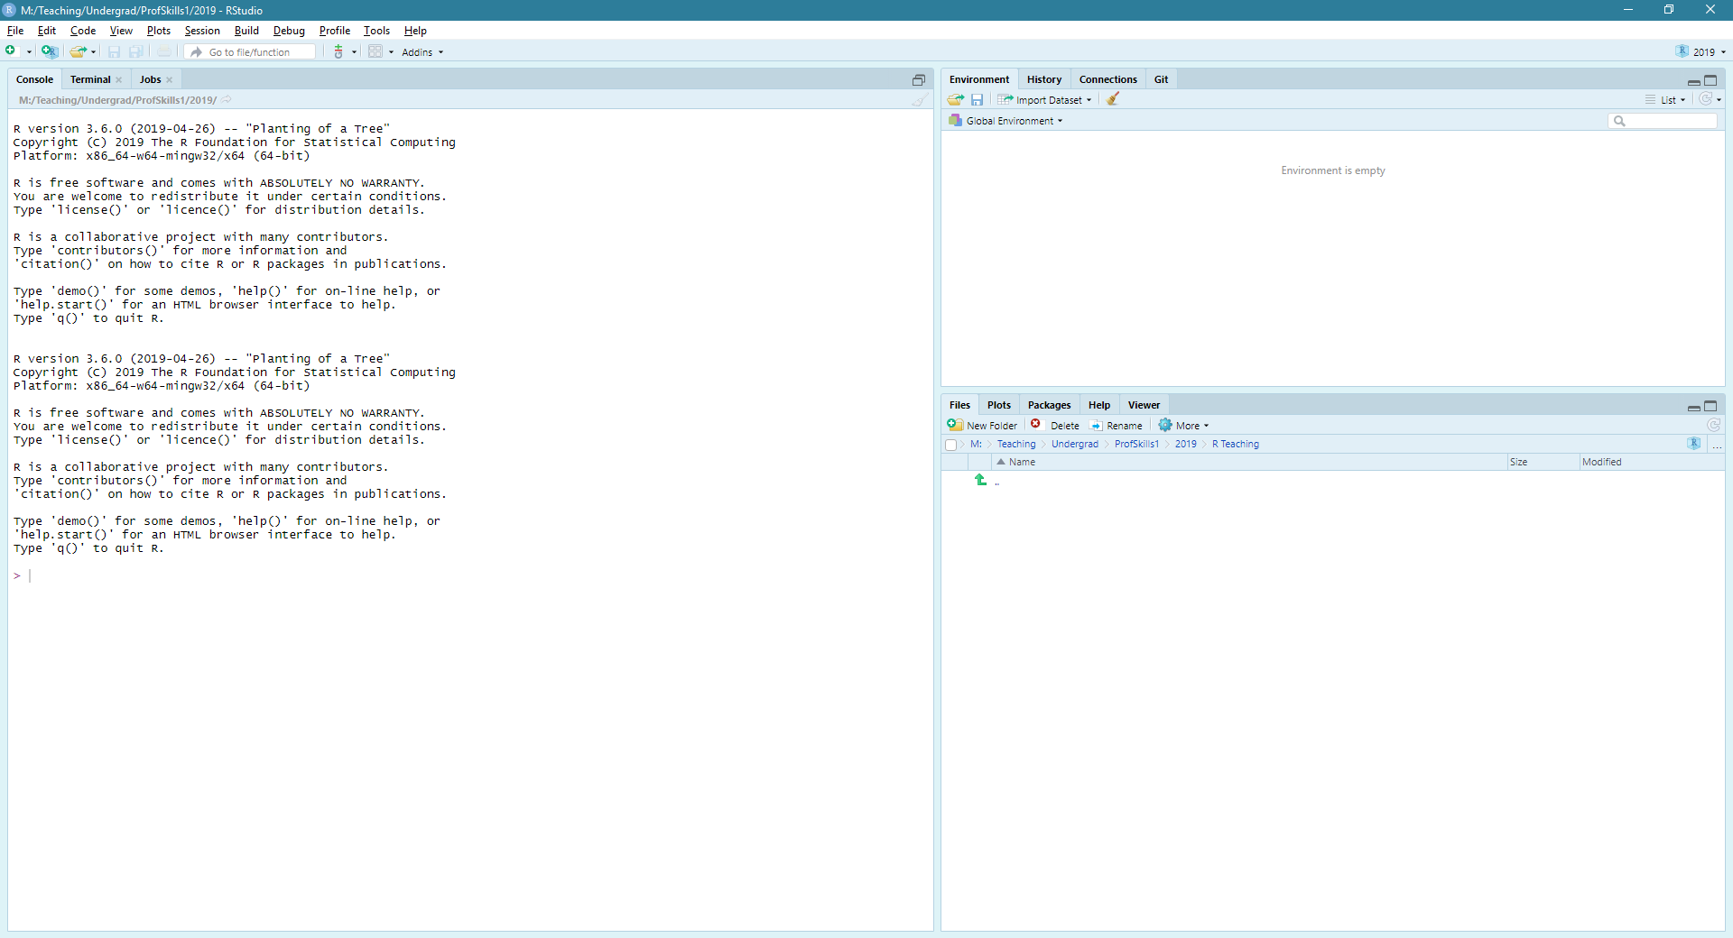
\includegraphics{images/02_install/rstud01} 

}

\caption{R Studio Overview}\label{fig:unnamed-chunk-6}
\end{figure}

\hypertarget{click-on-file-new-file-r-script}{%
\subsubsection{Click on File \textgreater{} New File\textgreater{} R Script}\label{click-on-file-new-file-r-script}}

Now your screen should look like \textbf{Figure 1.2}. You will have four panes in your window, and each pane can be dragged around or minimised. Note - you want to create a new R Script file, \textbf{not} an R Markdown or R Notebook file. We will do that next.

\begin{figure}

{\centering 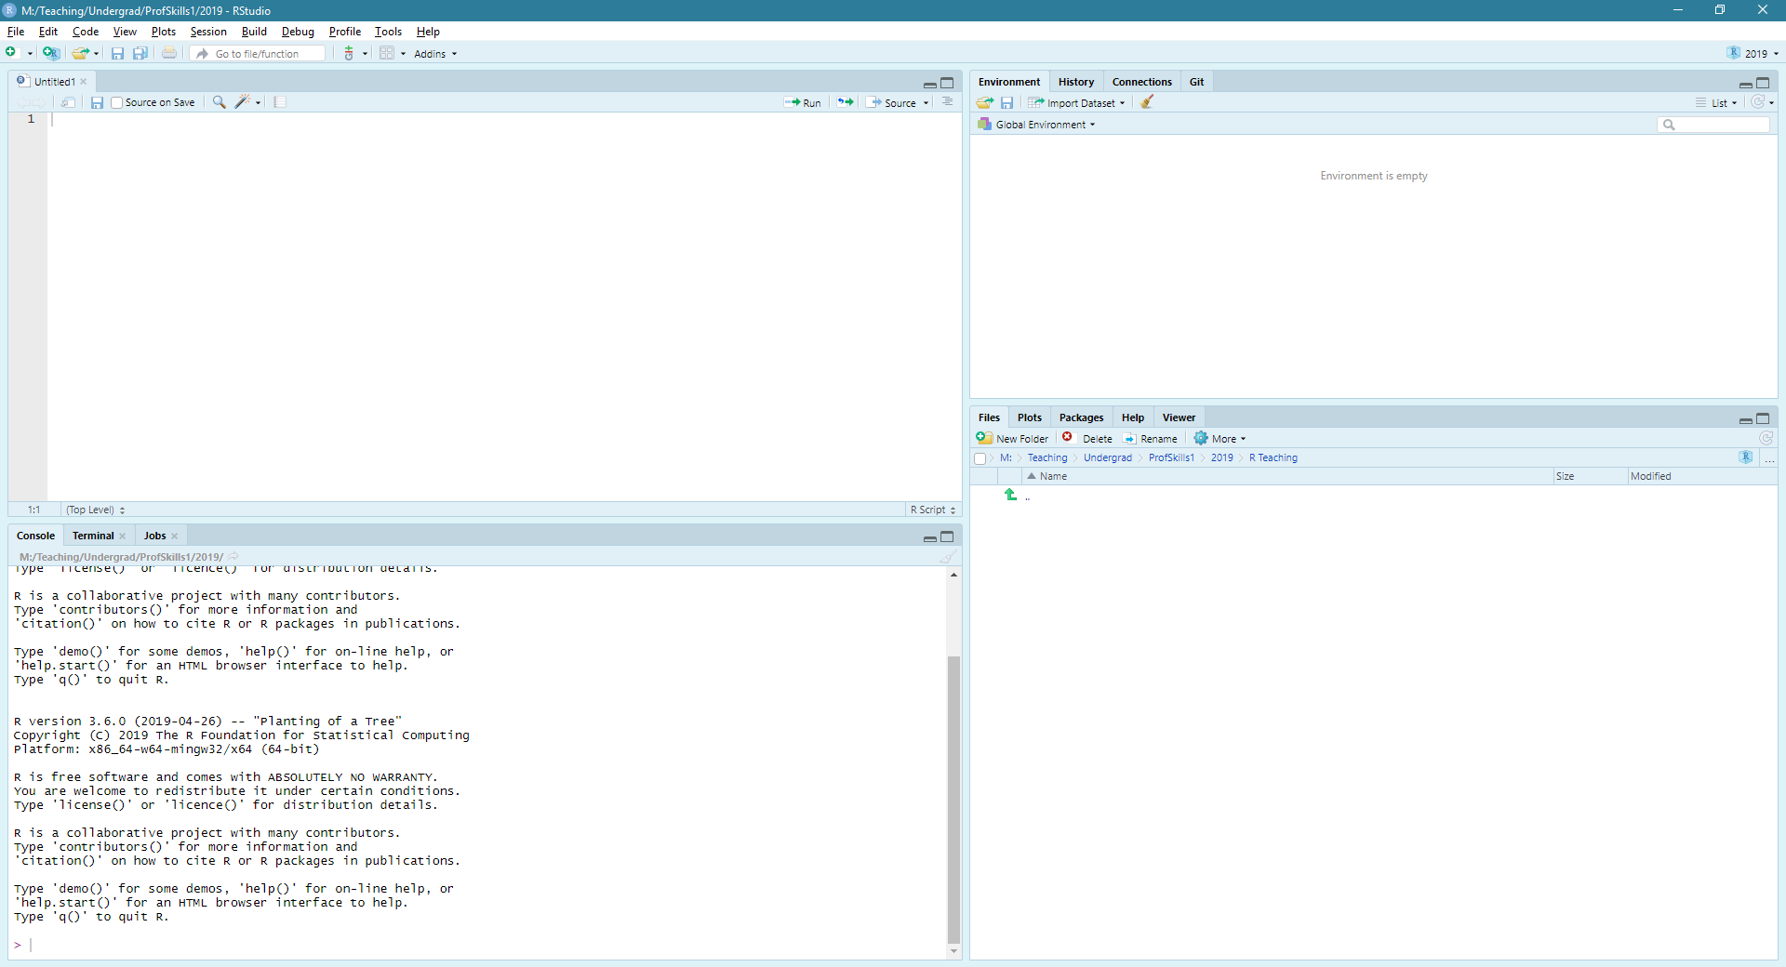
\includegraphics{images/02_install/rstud02} 

}

\caption{R Studio Overview with Script File}\label{fig:unnamed-chunk-7}
\end{figure}

\hypertarget{the-file-pane}{%
\subsubsection{The file pane}\label{the-file-pane}}

On the top left hand side of the R Studio window you can view the untitled R Script file you have just opened (\textbf{Figure 1.3}). Here you will see views of your files (mostly R Script files and R Markdown files in this book), and views of your data.

\begin{figure}

{\centering 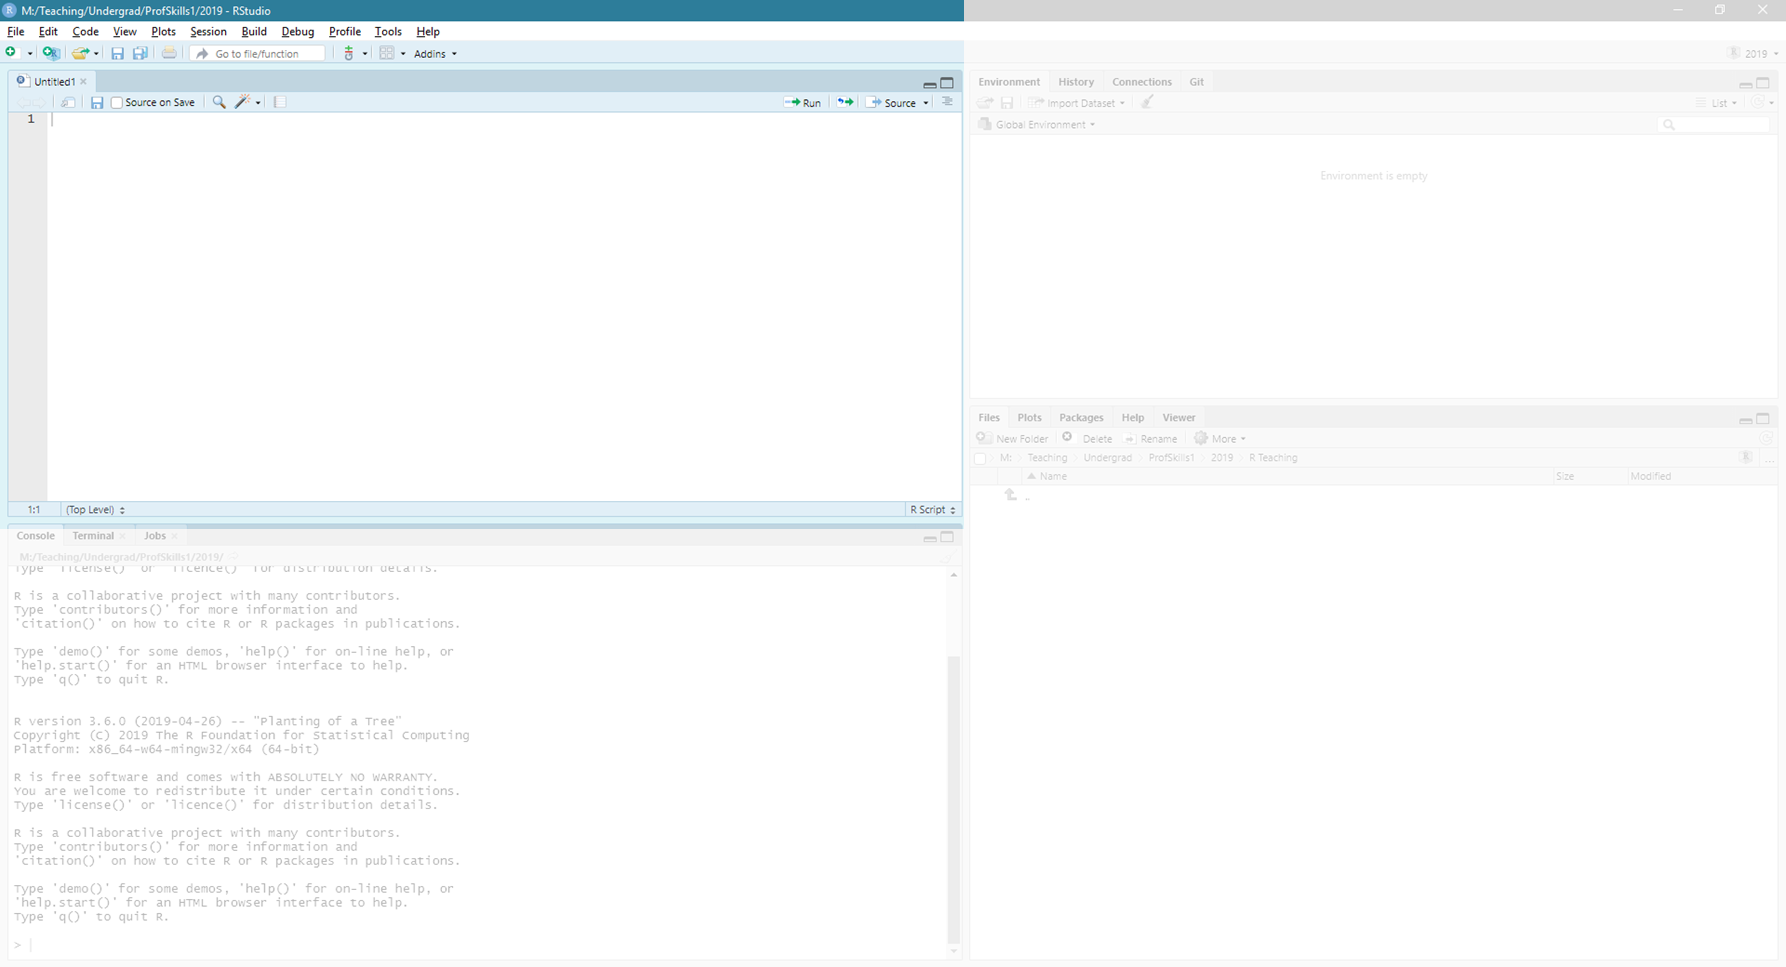
\includegraphics{images/02_install/rstud03} 

}

\caption{The active file pane}\label{fig:unnamed-chunk-8}
\end{figure}

\hypertarget{the-console}{%
\subsubsection{The console}\label{the-console}}

If you were using plain R (without R Studio) this console window is all you would see. Where you see this \textbf{\textgreater{}} symbol in the console you can type in a simple maths equation.

I recommend you type something now, perhaps \texttt{2\ +\ 2}

When you have finished typing, hit enter on your keyboard and see what the answer is.

Type \texttt{2\ +} and then hit enter. What happens? You will need to hit `escape' (`esc') on your keyboard to make the \textbf{\textgreater{}} symbol appear again.

Hitting `enter' asks R to perform the last command. Because we didn't tell R what it had to add, it kept waiting to find out what would come next.

\begin{figure}

{\centering 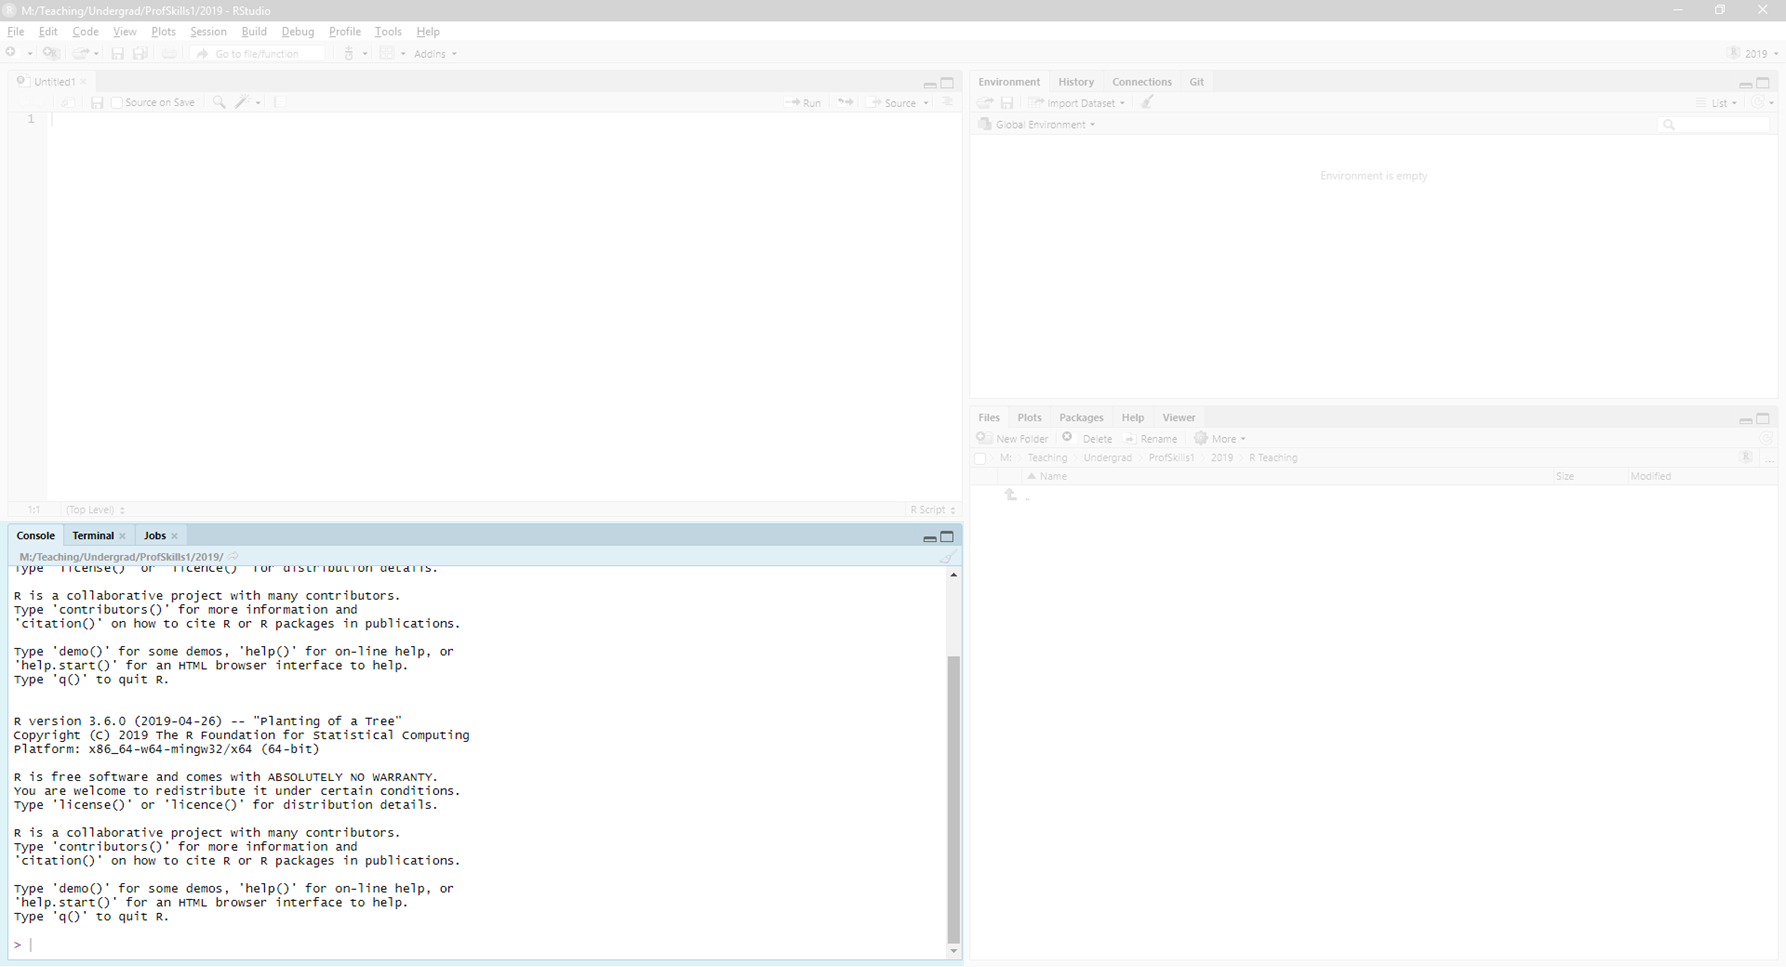
\includegraphics{images/02_install/rstud04} 

}

\caption{The console pane}\label{fig:unnamed-chunk-9}
\end{figure}

\hypertarget{the-environment-pane}{%
\subsubsection{The Environment pane}\label{the-environment-pane}}

The Environment is shown in \textbf{Figure 1.5}. At the moment, your environment will be empty. We will talk more about what goes here in \protect\hyperlink{environment}{the environment section of getting started}.

\begin{figure}

{\centering 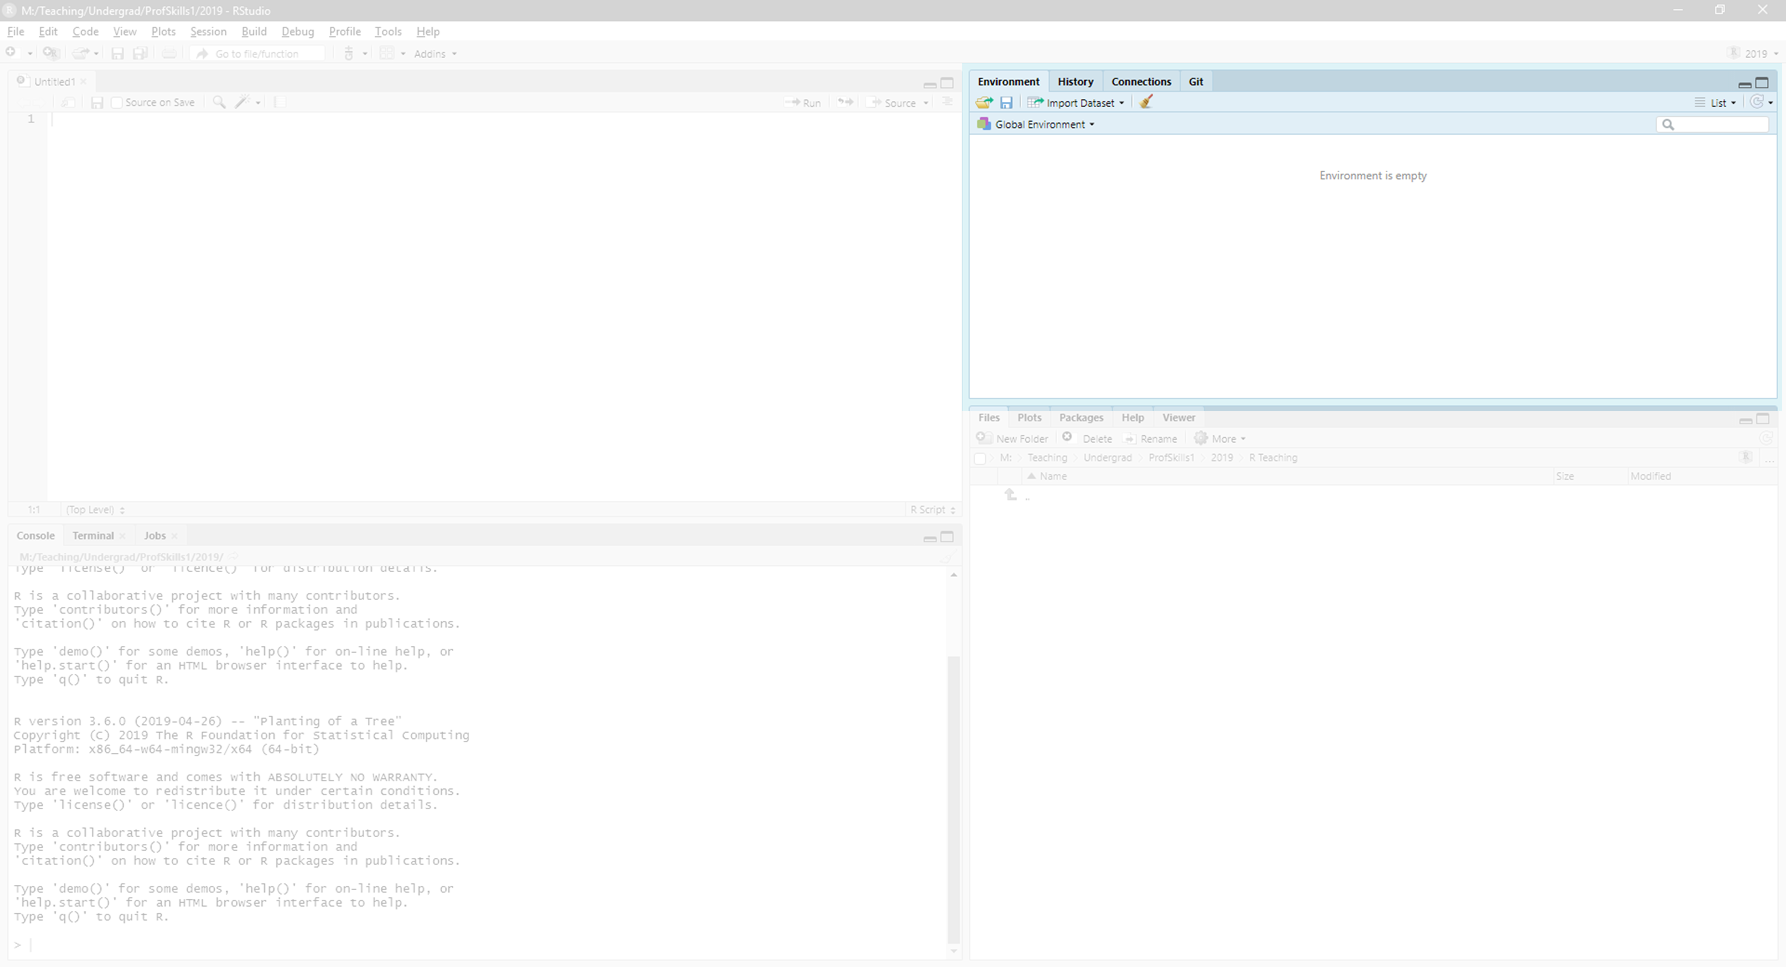
\includegraphics{images/02_install/rstud05} 

}

\caption{The environment pane}\label{fig:unnamed-chunk-10}
\end{figure}

\hypertarget{files-plots-packages-help-and-viewer}{%
\subsubsection{Files, plots, packages, help and viewer}\label{files-plots-packages-help-and-viewer}}

The final pane, shown in \textbf{Figure 1.6}, has five tabs in it by default.

These are:

\begin{itemize}
\tightlist
\item
  Files

  \begin{itemize}
  \tightlist
  \item
    Think of this like a Windows Explorer window (folder window) on your PC. It will show you all the files in your current folder and may just show your .Rproj file right now.
  \end{itemize}
\item
  Plots

  \begin{itemize}
  \tightlist
  \item
    When we start drawing charts they'll be saved here.
  \end{itemize}
\item
  Packages

  \begin{itemize}
  \tightlist
  \item
    Other wonderful people in the R Community write lots of clever code that can be `packaged' up so we can use it. Instead of writing out all the code you need to make a chart, you can use someone's package instead. We will learn more about these in \protect\hyperlink{packages}{packages}
  \end{itemize}
\item
  Help

  \begin{itemize}
  \tightlist
  \item
    If you ever get stuck with a commaned you can type \texttt{?command\_name} to view the command's documentation. Try it now by type \texttt{?summary} in the \textbf{console} window. Remember you need to press enter on your keyboard after typing the command.
  \end{itemize}
\item
  Viewer

  \begin{itemize}
  \tightlist
  \item
    This tab will show you more complicated things, like if you use R to build an html page (or a book like this one!) Ignore it for now.
  \end{itemize}
\end{itemize}

\begin{figure}

{\centering 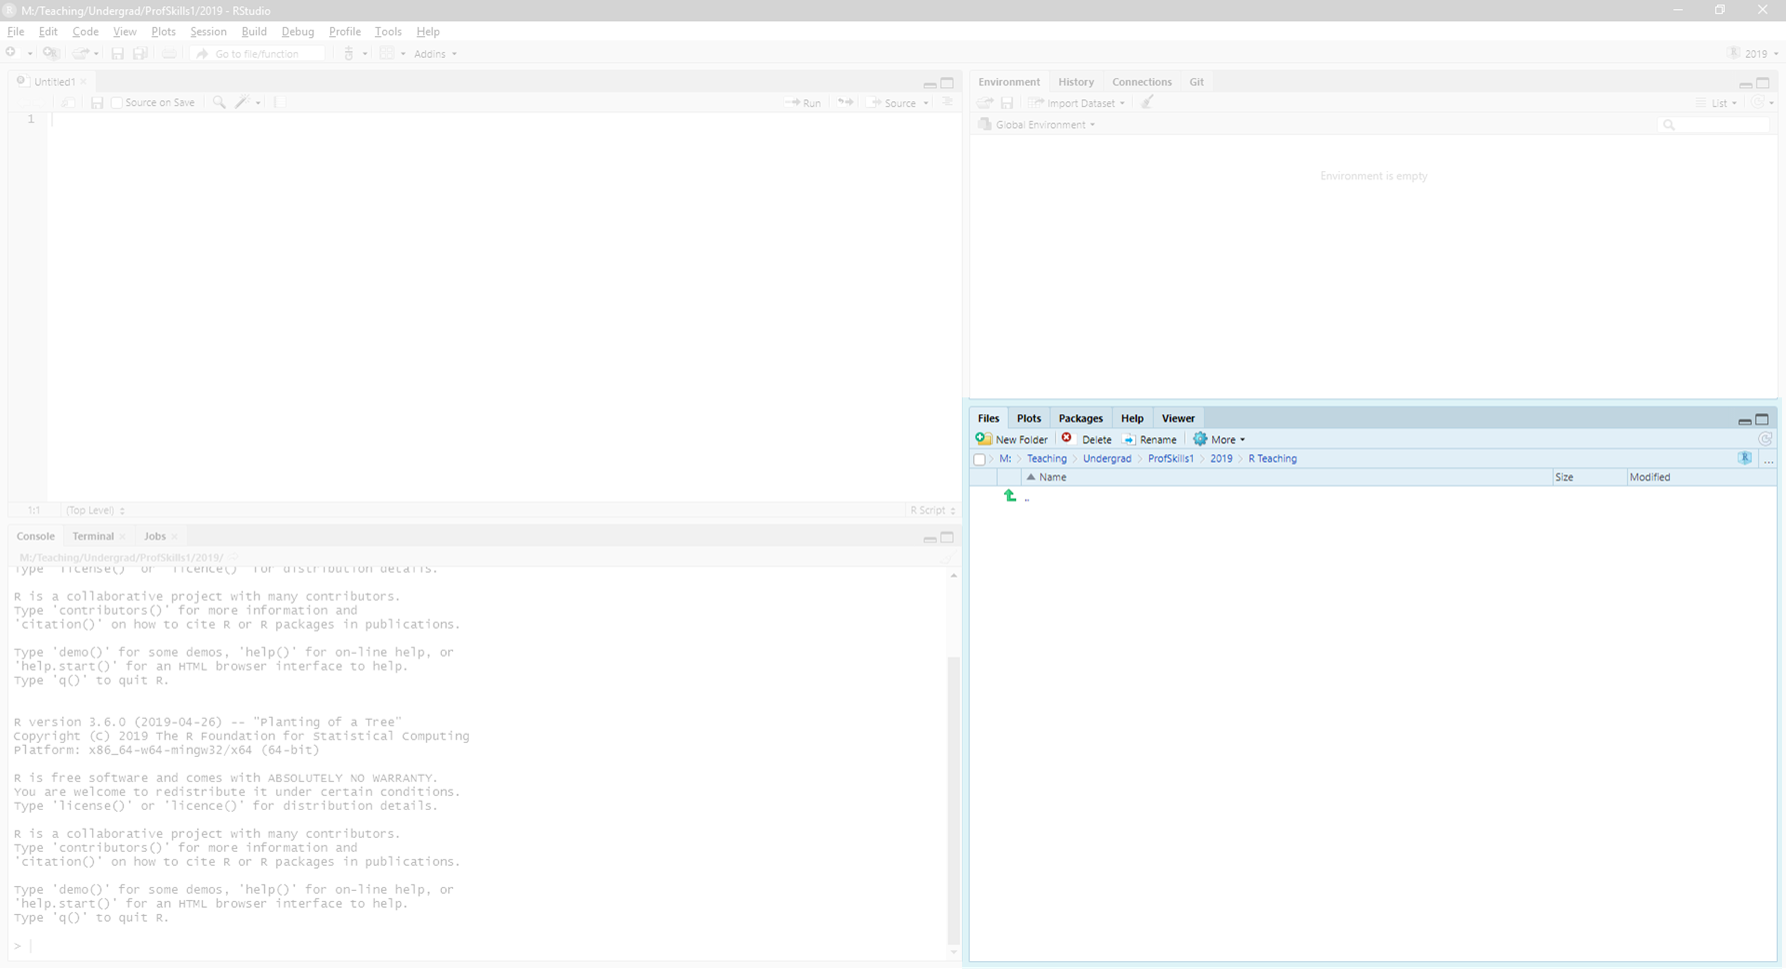
\includegraphics{images/02_install/rstud06} 

}

\caption{File, plot, package and help viewer}\label{fig:unnamed-chunk-11}
\end{figure}

\hypertarget{customisation}{%
\subsubsection{Customisation}\label{customisation}}

Data analysis is fun, and its also personal. You can customise your R Studio to look the way you want it to.

Go to \texttt{Tools\ \textgreater{}\ Global\ Options} (\textbf{Figure 1.7})

\begin{figure}

{\centering 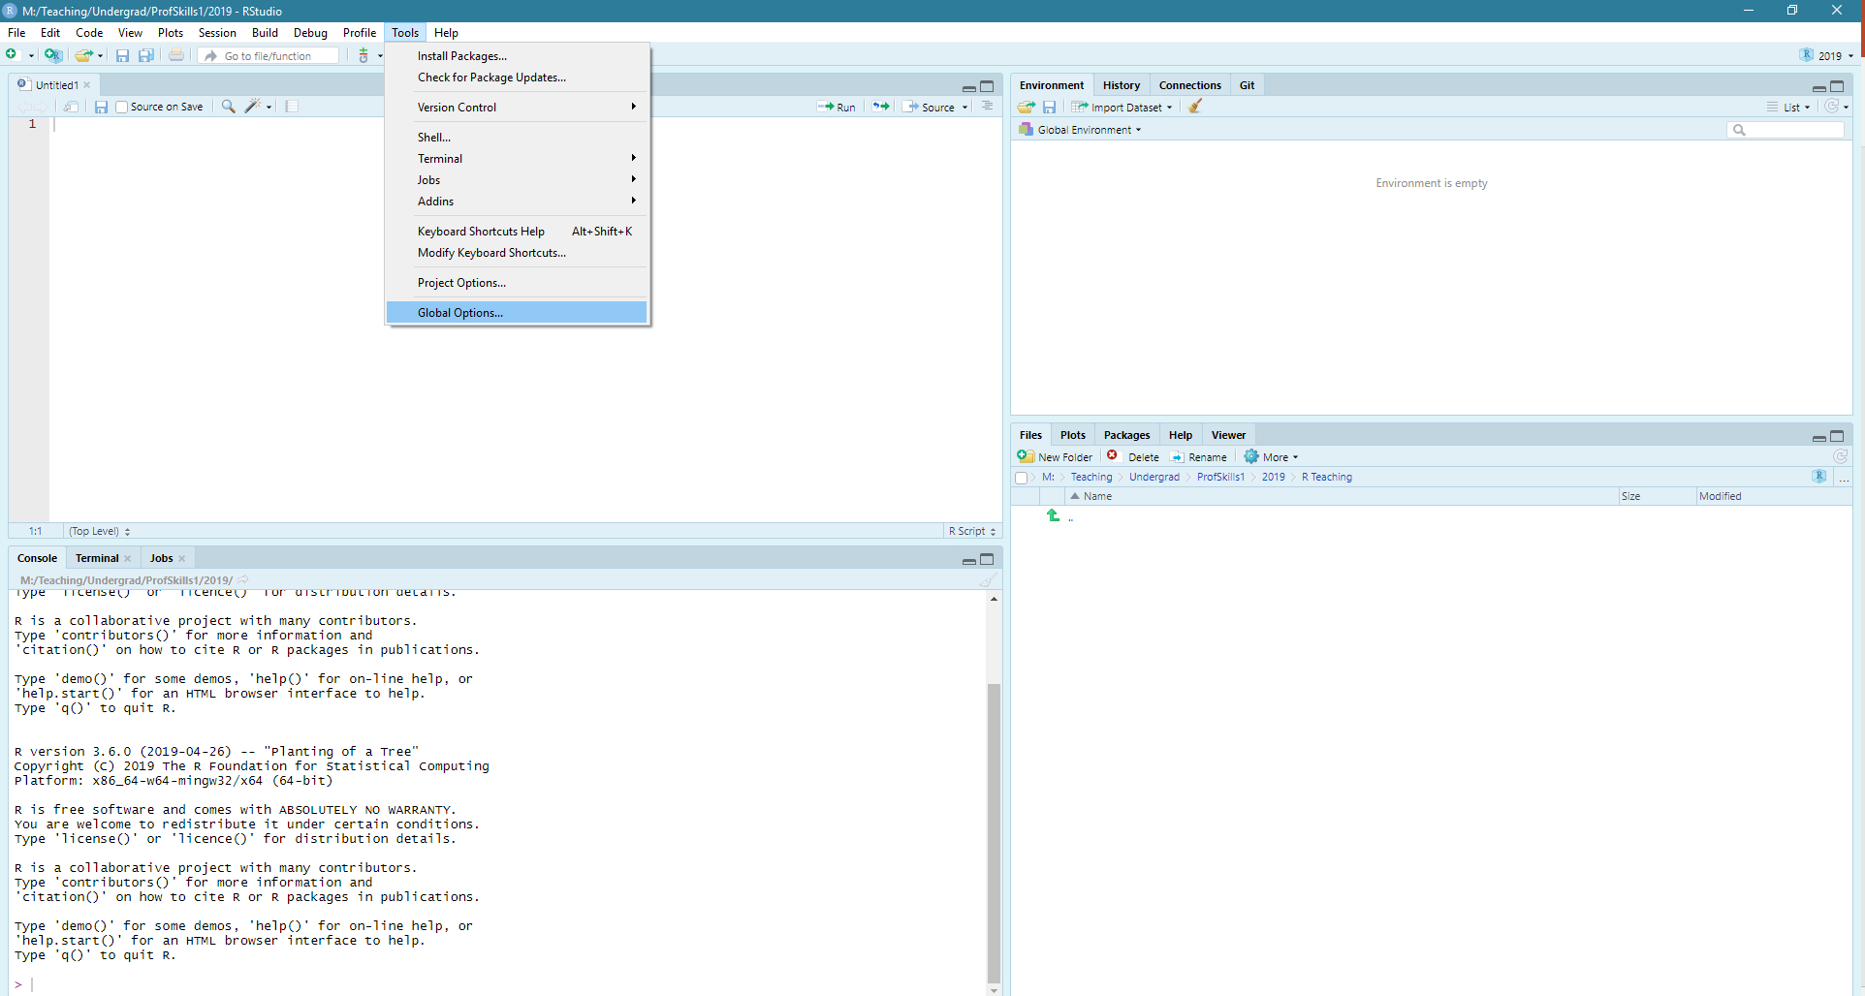
\includegraphics{images/02_install/rstud07} 

}

\caption{Global options}\label{fig:unnamed-chunk-12}
\end{figure}

And then go to \texttt{Appearance\ \textgreater{}\ Editor\ Theme} to play around and find the colour scheme, font, and R Studio Theme you like best (\textbf{Figure 1.8})

\begin{figure}

{\centering 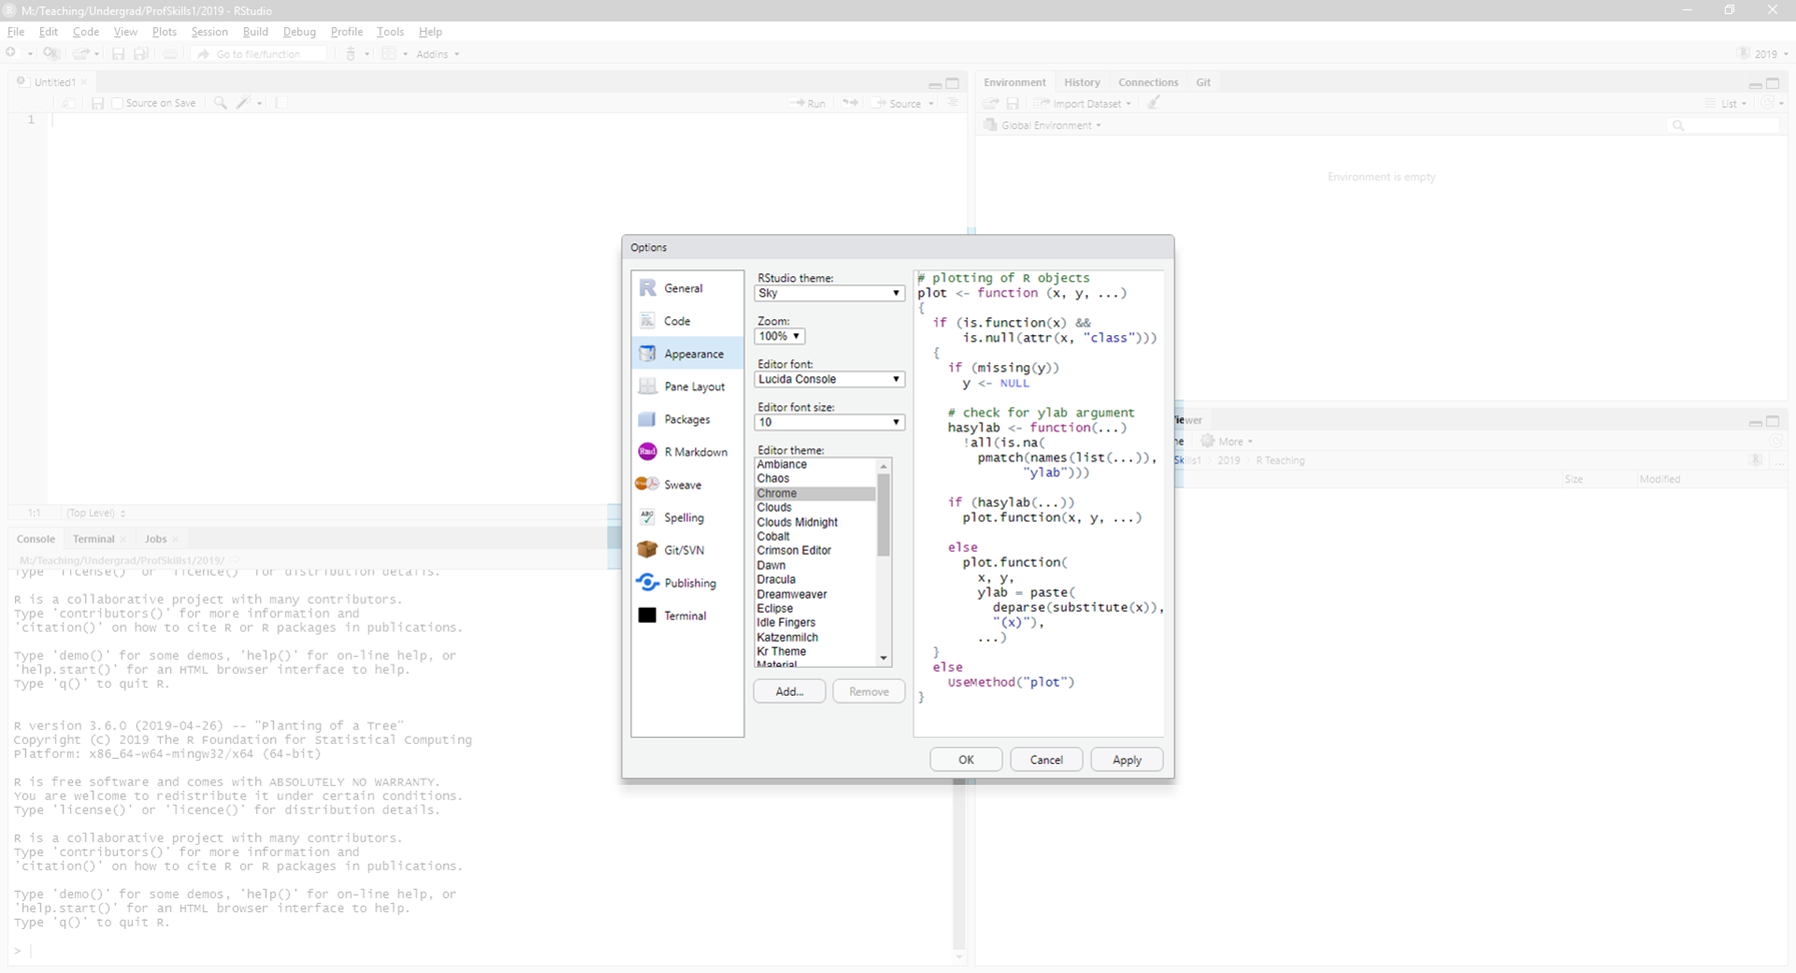
\includegraphics{images/02_install/rstud08} 

}

\caption{Global options, themes}\label{fig:unnamed-chunk-13}
\end{figure}

Personally I like the theme \texttt{XCode}, but it's your R Studio! You choose the one you like.

\hypertarget{install_rsc}{%
\section{Using the Cloud}\label{install_rsc}}

If you would like to use R Studio Cloud, you will need to create an R Studio account. This can be a whole new account, a google account, or a github account. I would recommend you get a github account (you can jump \protect\hyperlink{github}{to read why here}).

After you have logged in, you can access a workspace. A workspace is like an R Studio Project.

As of the 3rd August, 2020, R Studio Cloud is moving out of Beta and will be available to all. You should use the \textbf{Cloud Free Plan}. Again, we do not expect you to buy anything to use R or R Studio.

You will have a maximum of 15 projects you can use, and less storage space than using your own device.

\hypertarget{install_vids}{%
\section{Install R and R Studio - Video Instruction}\label{install_vids}}

If you prefer to get your resources in video format, there's an explanation of \href{https://media.ed.ac.uk/media/R+ConversationsA+Installing+R+and+R+Studio/1_q0mdj8mk/104843251}{installing R and R Studio here} and using \href{https://media.ed.ac.uk/media/R+ConversationsA+R+Studio+Online/1_ex8u0oj7/112983051}{R Studio Cloud here}.

Please note, these videos are a bit older now so you should expect to see some minor differences, e.g.~in version numbers.

\hypertarget{start}{%
\chapter{Getting Started}\label{start}}

\begin{quote}
You can skip this chapter if you can:

\begin{itemize}
\item
  Use the console to input simple lines of code
\item
  Install and load a package
\item
  Know what a function is
\end{itemize}
\end{quote}

To use this chapter you will need a working version of R and R Studio.

If you can open R Studio and type \texttt{2\ +\ 2} in the \textbf{console} you are good to go.

If that is confusing, you might need to jump back to \protect\hyperlink{install_rs}{installing R Studio} and the section \protect\hyperlink{navigate_rs}{navigating R Studio}.

\hypertarget{thesecret}{%
\section{The Big Secret}\label{thesecret}}

Okay. This is the Big Secret. The thing you will not believe. The most important thing you'll learn about R.

You should copy and paste other peoples' code.

Yes, I'm serious. You should copy and paste and edit code you find online\footnote{If you're reading this as part of your coursework you might be panicking about plagiarism here, after all, we spend a lot of time telling you plagiarism is the worst thing you could ever do and that we'll use software to detect it. Code is a bit different. We are always trying to find the most efficient way of doing something, and so ideally you would all write code that was identical. Sadly, humans naturally differ in the way the think about problems. My job would be a lot easier if everybody thought the same. If I have set you this book as reading, I can swear to you I will never put your code through a plagiarism checker. That would be very stupid.}. In this book you should always be copying bits of code and pasting it into your console. That is why I publish the code alongside it.

It took me about ten years of working in R to get over my fear of copying and pasting other peoples' code. Now I even have a \href{https://github.com/jillymackay/commoncode}{repository} of all the code I use over and over so I can copy and paste my own code.

Most people will not remember code off the top of their head. This is why we use the help function (remember \texttt{?summary}) to look at the documentation, and resources like Stack Exchange and Google to help us (more in \protect\hyperlink{trouble}{troubleshooting}).

\hypertarget{ex_tidytuesday}{%
\subsection{Exercise}\label{ex_tidytuesday}}

You might be very skeptical here about how much I want you to be copying code. If you're not convinced, I suggest you go watch my RStats Crush the amazing \href{https://twitter.com/drob}{David Robinson} do one of his Tidy Tuesday screencasts. David Robinson has forgotten more R than I'll ever learn, and see - he still \href{https://www.youtube.com/channel/UCeiiqmVK07qhY-wvg3IZiZQ}{copies and pastes code}.

\hypertarget{projects}{%
\section{Projects}\label{projects}}

I would like to being by creating a new project in R Studio.

\begin{itemize}
\item
  Open R Studio
\item
  Go to \texttt{File\ \textgreater{}\ New\ Project}
\item
  Set up a new project either in an existing directory (folder), or in a new one. Ignore repositories for now.
\end{itemize}

You can call this project anything you like. I recommend something short like `start'.

A R Project sits inside a folder. Everything inside that folder is part of that R Project. Let's say you have a folder called:

\texttt{mydata}

and you create an R Project called \texttt{analysis}.

The \texttt{analysis.Rproj} will live inside the \texttt{mydata} folder, and it will `see' all the data, files, and any other folders, you have in \texttt{mydata}.

Using R Studio you will get a lot better at `directory management', or knowing where you have saved things.

\hypertarget{environment}{%
\section{Environment}\label{environment}}

In your brand new project you will have a clean environment (refer back to \protect\hyperlink{navigate_rs}{Figure 2.5}). Our first exercise is going to explore what the environment really means.

\hypertarget{ex_env}{%
\subsection{Exercise - Environment}\label{ex_env}}

When we first installed R, you were typing mathematical equations into the console. Let's remind ourselves of this by running an equation now. In the console, type a long and complicated equation, then hit `enter' when you're done.

\begin{Shaded}
\begin{Highlighting}[]
\DecValTok{500} \OperatorTok{+}\StringTok{ }\DecValTok{23} \OperatorTok{/}\StringTok{ }\DecValTok{91}
\end{Highlighting}
\end{Shaded}

\begin{verbatim}
## [1] 500.2527
\end{verbatim}

If this was a calculation we often ran, we might want to save the answer. We can do this by using the \textbf{assign} symbol \textbf{\textless{}-}.

For example, if we type this:

\begin{Shaded}
\begin{Highlighting}[]
\NormalTok{x <-}\StringTok{ }\DecValTok{500} \OperatorTok{+}\StringTok{ }\DecValTok{23} \OperatorTok{/}\StringTok{ }\DecValTok{91}
\end{Highlighting}
\end{Shaded}

\ldots{} you will see that we simply get a new line returned. We don't get the answer. However, in your environment you will see under the heading `Values', a new thing called \texttt{x}.

Enter the following code:

\begin{Shaded}
\begin{Highlighting}[]
\NormalTok{x}
\end{Highlighting}
\end{Shaded}

\begin{verbatim}
## [1] 500.2527
\end{verbatim}

R remembers what x is and recalled it. This is useful if we want to do more with \texttt{x} after we've calculated it.

\begin{Shaded}
\begin{Highlighting}[]
\NormalTok{x }\OperatorTok{/}\DecValTok{100}
\end{Highlighting}
\end{Shaded}

\begin{verbatim}
## [1] 5.002527
\end{verbatim}

As well as values, we can ask R to remember a string of text as well. Try this:

\begin{Shaded}
\begin{Highlighting}[]
\NormalTok{hello <-}\StringTok{ "Computers always print 'Hello World!' but we never say hello back"}


\KeywordTok{print}\NormalTok{(hello)}
\end{Highlighting}
\end{Shaded}

\begin{verbatim}
## [1] "Computers always print 'Hello World!' but we never say hello back"
\end{verbatim}

But R is very fussy. What happens if you run this code:

\begin{Shaded}
\begin{Highlighting}[]
\KeywordTok{print}\NormalTok{(HELLO)}
\end{Highlighting}
\end{Shaded}

You see, R ise \textbf{case sensitive}, meaning we have to be careful to always type things the same. This is one of the reasons why R Studio is really handy, because you can see what you've saved in your environment.

Now type this:

\begin{Shaded}
\begin{Highlighting}[]
\NormalTok{hello <-}\StringTok{ "Hello, R!"}
\end{Highlighting}
\end{Shaded}

Take a guess what is going to happen before you type the next line. Were you right?

\begin{Shaded}
\begin{Highlighting}[]
\KeywordTok{print}\NormalTok{(hello)}
\end{Highlighting}
\end{Shaded}

\begin{verbatim}
## [1] "Hello, R!"
\end{verbatim}

\hypertarget{ex_func}{%
\subsection{Exercise - Functions}\label{ex_func}}

\hypertarget{the-basic-function}{%
\subsubsection{The Basic Function}\label{the-basic-function}}

A function is a handy way to bundle together some lines of code. David Robinson \href{https://twitter.com/drob/status/928447584712253440?s=20}{says that} if you run a few lines more than twice you should write a function to do it instead.

I'm going to contradict myself now. Functions are really important in R, but I'm not going to ask you to write one anywhere else but in this exercise. Most things in this book I expect you to practice over and over, but functions are useful to understand \protect\hyperlink{packages}{packages}, and that's why we're going to talk about them now.

Let's create a function to make R welcome us. Copy and paste this code into a new script file (you may want to save it as your functions example), and then run it.

\begin{Shaded}
\begin{Highlighting}[]
\NormalTok{mynameis <-}\StringTok{ }\ControlFlowTok{function}\NormalTok{ (name) \{}
  \KeywordTok{print}\NormalTok{ (}\KeywordTok{paste0}\NormalTok{(}\StringTok{"Hello, "}\NormalTok{, name, }\StringTok{", how are you today?"}\NormalTok{))}
\NormalTok{\}}
\KeywordTok{mynameis}\NormalTok{ (}\StringTok{"Jill"}\NormalTok{)}
\end{Highlighting}
\end{Shaded}

\begin{verbatim}
## [1] "Hello, Jill, how are you today?"
\end{verbatim}

You may have noticed that, just like when we were assigning \texttt{x} a value, we now have something in our environment called \texttt{mynameis}.

Whenever we type \texttt{mynameis("Jill")} into the console, or execute that line in a script file, R knows it should look to the environment and run the code that's been bundled up into that package.

For example, we could make R welcome us in exactly the same way by typing:

\begin{Shaded}
\begin{Highlighting}[]
\KeywordTok{print}\NormalTok{ (}\KeywordTok{paste0}\NormalTok{(}\StringTok{"Hello, "}\NormalTok{, }\StringTok{"Jill"}\NormalTok{, }\StringTok{", how are you today?"}\NormalTok{))}
\end{Highlighting}
\end{Shaded}

\begin{verbatim}
## [1] "Hello, Jill, how are you today?"
\end{verbatim}

But we would need to change the name every time we wanted welcome a new user. We are lazy, so we use the function to reduce the amount of things we need to change to get a different outcome.

Functions make our code more standardised. If we all define the \texttt{mynameis} function at the start of our documentation, we don't need to worry about accidentally deleting an important character in the code. This is especially important as we like to copy-paste code when we need to.

Most scientists will probably not write their own functions, but you should know how they work.

\hypertarget{packages}{%
\section{Packages}\label{packages}}

If people write very good and useful functions, they usually want to share them. They can do this with packages.

There are packages for everything, packages for drawing maps, packages for analysing data, packages for suggesting how to analyse your data, packages to give you more data, packages for tidying your data . . . this is one of the reasons we might all have different bits of code. There can be lots of ways to do something.

\hypertarget{ex_packages}{%
\subsection{Exercise - Install and Load a Package}\label{ex_packages}}

Packages work in two stages. The very first time you need a package you need to install it. Then, every time you start R you need to load the package into your livrary.

To install a package you need to type \texttt{install.package("package\_name")}.

To load it into your library you need to type \texttt{library(package\_name)}.

When you load a package from your library it goes into a special hidden environment where you can access all the functions that the package has written for you.

For example, we will make great use of the \texttt{tidyverse} package in this book. You need to start by installing it with:

\begin{Shaded}
\begin{Highlighting}[]
\KeywordTok{install.packages}\NormalTok{(}\StringTok{"tidyverse"}\NormalTok{)}
\end{Highlighting}
\end{Shaded}

And when it has finished downloading, you need to type:

\begin{Shaded}
\begin{Highlighting}[]
\KeywordTok{library}\NormalTok{(tidyverse)}
\end{Highlighting}
\end{Shaded}

to load it. You'll see that nothing has appeared in your Environment, but actually you have a whole host of new functions \& data you can play with. For example:

\begin{Shaded}
\begin{Highlighting}[]
\KeywordTok{slice}\NormalTok{(starwars)}
\end{Highlighting}
\end{Shaded}

Which should give you this:

\begin{verbatim}
## Warning: `...` is not empty.
## 
## We detected these problematic arguments:
## * `needs_dots`
## 
## These dots only exist to allow future extensions and should be empty.
## Did you misspecify an argument?
\end{verbatim}

\begin{verbatim}
## # A tibble: 87 x 14
##    name     height  mass hair_color  skin_color  eye_color birth_year sex   gender homeworld species films vehicles starships
##    <chr>     <int> <dbl> <chr>       <chr>       <chr>          <dbl> <chr> <chr>  <chr>     <chr>   <lis> <list>   <list>   
##  1 Luke Sk~    172    77 blond       fair        blue            19   male  mascu~ Tatooine  Human   <chr~ <chr [2~ <chr [2]>
##  2 C-3PO       167    75 <NA>        gold        yellow         112   none  mascu~ Tatooine  Droid   <chr~ <chr [0~ <chr [0]>
##  3 R2-D2        96    32 <NA>        white, blue red             33   none  mascu~ Naboo     Droid   <chr~ <chr [0~ <chr [0]>
##  4 Darth V~    202   136 none        white       yellow          41.9 male  mascu~ Tatooine  Human   <chr~ <chr [0~ <chr [1]>
##  5 Leia Or~    150    49 brown       light       brown           19   fema~ femin~ Alderaan  Human   <chr~ <chr [1~ <chr [0]>
##  6 Owen La~    178   120 brown, grey light       blue            52   male  mascu~ Tatooine  Human   <chr~ <chr [0~ <chr [0]>
##  7 Beru Wh~    165    75 brown       light       blue            47   fema~ femin~ Tatooine  Human   <chr~ <chr [0~ <chr [0]>
##  8 R5-D4        97    32 <NA>        white, red  red             NA   none  mascu~ Tatooine  Droid   <chr~ <chr [0~ <chr [0]>
##  9 Biggs D~    183    84 black       light       brown           24   male  mascu~ Tatooine  Human   <chr~ <chr [0~ <chr [1]>
## 10 Obi-Wan~    182    77 auburn, wh~ fair        blue-gray       57   male  mascu~ Stewjon   Human   <chr~ <chr [1~ <chr [5]>
## # ... with 77 more rows
\end{verbatim}

Now we have a new dataset (\texttt{starwars}) and a new thing we can do (\texttt{slice} the top of the data). We will talk much more about \texttt{tidyverse} in the \protect\hyperlink{data}{data chapter}.

\hypertarget{scripts_rmd}{%
\section{R Markdown vs R Scripts}\label{scripts_rmd}}

\hypertarget{video_rmd}{%
\subsection{A video on R Markdown}\label{video_rmd}}

If you would like to watch me using R Markdown, you're in luck! Theres \href{https://media.ed.ac.uk/media/R+ConversationsA+Intro+to+R+Markdown/1_td0q33v8/112983051}{a video here}.

\hypertarget{video_env}{%
\section{Video Introductions}\label{video_env}}

There is a short introduction to R and R Studio in Video format here:

\begin{itemize}
\item
  \href{https://media.ed.ac.uk/media/R+ConversationsA+Intro+to+R+Studio+1/1_aox3in51/112983051}{Video 1}
\item
  \href{https://media.ed.ac.uk/media/R+ConversationsA+Intro+to+R+Studio+2/1_vm1bylon}{Video 2}
\end{itemize}

\hypertarget{data}{%
\chapter{Data}\label{data}}

\begin{quote}
You can skip this chapter if you:

\begin{itemize}
\item
  Are comfortable working with dataframes and tibbles
\item
  Know about and are comfortable using some of R's inbuilt data packages
\item
  Are comfortable loading .csv and .xlsx files into R
\end{itemize}
\end{quote}

\hypertarget{packages-for-this-chapter}{%
\section{Packages for this chapter}\label{packages-for-this-chapter}}

In this chapter you'll want the following packages loaded in your R session. At the start, you will need to run the following code. Remember if you don't have a package you can install it with the \texttt{install.package("package\_name")} command.

\begin{Shaded}
\begin{Highlighting}[]
\KeywordTok{library}\NormalTok{(tidyverse)}
\KeywordTok{library}\NormalTok{(readxl)}
\end{Highlighting}
\end{Shaded}

\hypertarget{data_builtin}{%
\section{Built In Data}\label{data_builtin}}

Many packages, such as the \texttt{tidyverse} package, and the default\footnote{`Default' here means one you won't need to install or load into the library} \texttt{datasets} package come with data in them. These datasets can be really useful for testing code that you're unfamiliar with, because you know what the data should look like, and how it should perform.

Some common datasets are:

\begin{itemize}
\item
  \texttt{mpg}

  \begin{itemize}
  \tightlist
  \item
    Fuel economy data from 1999 to 2008 for 38 popular models of cars
  \end{itemize}
\item
  \texttt{ChickWeight}
\item
  Weight versus age of chicks on different diets
\item
  \texttt{starwars}

  \begin{itemize}
  \tightlist
  \item
    Name, height, weight, age, and other characteristics of Star Wars characters
  \end{itemize}
\item
  \texttt{iris}

  \begin{itemize}
  \tightlist
  \item
    The measurements (in cm) of the sepal length and width and petal length and width of 50 flowers in 3 species of iris
  \end{itemize}
\end{itemize}

There are many, many more. You can explore some of them by typing \texttt{datasets::}\footnote{You might wonder, what's the \texttt{::} in the \texttt{datasets::} command. The \texttt{::} is very useful and tells R to look inside the \texttt{datasets} package without having to actually load it into your library which can be very quick and easy} into the console and instead of pressing `enter', scroll the menu that pops up to help you autocomplete your command.

\hypertarget{ex_inbuiltdata}{%
\section{Exercise}\label{ex_inbuiltdata}}

For our first exercise we are going to look at some of the inbuilt datasets.

What happens when you enter the following code\footnote{If its not working - are you sure you have spelled it with a capital \texttt{View}?} into the console?

\begin{Shaded}
\begin{Highlighting}[]
\KeywordTok{View}\NormalTok{(mpg)}
\end{Highlighting}
\end{Shaded}

You should see something like \textbf{Figure 3.1}

\begin{figure}

{\centering 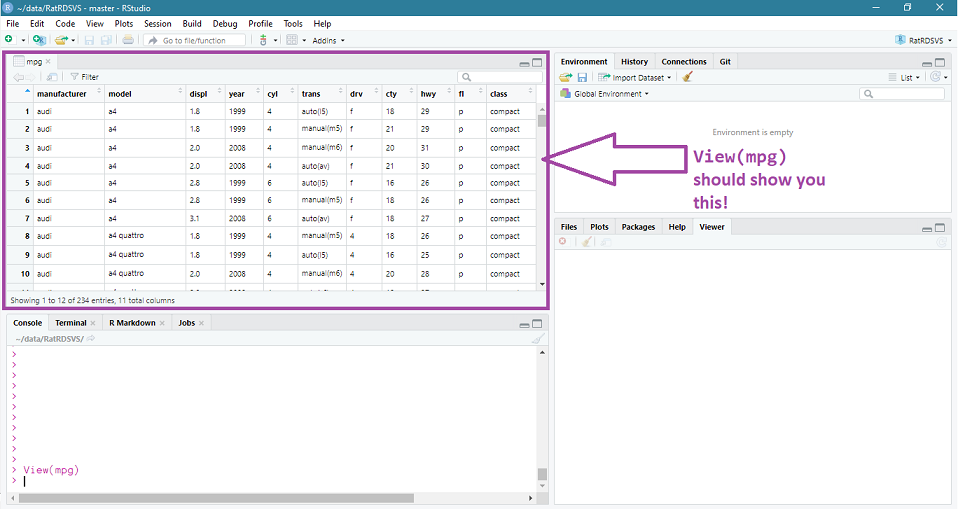
\includegraphics{images/03_data/rstud01} 

}

\caption{The result of the 'View(mpg)' command}\label{fig:unnamed-chunk-31}
\end{figure}

The \texttt{View()} command is very handy for getting a quick window onto what data looks like. Unfortunately, the \texttt{View()} command only really works for \textbf{you} getting a look at your data. If you wanted to share your code, you would be better using a command which prints some of the data into the console.

So - what functions will tell R to print data into the console?

You can view the top of a dataset with \texttt{head()}

\begin{Shaded}
\begin{Highlighting}[]
 \KeywordTok{head}\NormalTok{(mpg)}
\end{Highlighting}
\end{Shaded}

\begin{verbatim}
## # A tibble: 6 x 11
##   manufacturer model displ  year   cyl trans      drv     cty   hwy fl    class  
##   <chr>        <chr> <dbl> <int> <int> <chr>      <chr> <int> <int> <chr> <chr>  
## 1 audi         a4      1.8  1999     4 auto(l5)   f        18    29 p     compact
## 2 audi         a4      1.8  1999     4 manual(m5) f        21    29 p     compact
## 3 audi         a4      2    2008     4 manual(m6) f        20    31 p     compact
## 4 audi         a4      2    2008     4 auto(av)   f        21    30 p     compact
## 5 audi         a4      2.8  1999     6 auto(l5)   f        16    26 p     compact
## 6 audi         a4      2.8  1999     6 manual(m5) f        18    26 p     compact
\end{verbatim}

Note that this code has produced an output block. Unlike \texttt{View()} where I had to share a screengrab to show you what the output of the code was. This is why \texttt{head()} is a lot more reproducible than \texttt{View()} and should be your default for code sharing. See more about this in \protect\hyperlink{workflows}{workflows}.

Unsurprisingly we can also view the bottom of a dataset with \ldots{}

\begin{Shaded}
\begin{Highlighting}[]
\KeywordTok{tail}\NormalTok{(mpg)}
\end{Highlighting}
\end{Shaded}

\begin{verbatim}
## # A tibble: 6 x 11
##   manufacturer model  displ  year   cyl trans      drv     cty   hwy fl    class  
##   <chr>        <chr>  <dbl> <int> <int> <chr>      <chr> <int> <int> <chr> <chr>  
## 1 volkswagen   passat   1.8  1999     4 auto(l5)   f        18    29 p     midsize
## 2 volkswagen   passat   2    2008     4 auto(s6)   f        19    28 p     midsize
## 3 volkswagen   passat   2    2008     4 manual(m6) f        21    29 p     midsize
## 4 volkswagen   passat   2.8  1999     6 auto(l5)   f        16    26 p     midsize
## 5 volkswagen   passat   2.8  1999     6 manual(m5) f        18    26 p     midsize
## 6 volkswagen   passat   3.6  2008     6 auto(s6)   f        17    26 p     midsize
\end{verbatim}

Another very useful way to look at a dataset is with the \texttt{summary()} function, which takes its best guess at how to summarise each variable in the dataset.

\begin{Shaded}
\begin{Highlighting}[]
\KeywordTok{summary}\NormalTok{(mpg)}
\end{Highlighting}
\end{Shaded}

\begin{verbatim}
##  manufacturer          model               displ            year           cyl           trans               drv           
##  Length:234         Length:234         Min.   :1.600   Min.   :1999   Min.   :4.000   Length:234         Length:234        
##  Class :character   Class :character   1st Qu.:2.400   1st Qu.:1999   1st Qu.:4.000   Class :character   Class :character  
##  Mode  :character   Mode  :character   Median :3.300   Median :2004   Median :6.000   Mode  :character   Mode  :character  
##                                        Mean   :3.472   Mean   :2004   Mean   :5.889                                        
##                                        3rd Qu.:4.600   3rd Qu.:2008   3rd Qu.:8.000                                        
##                                        Max.   :7.000   Max.   :2008   Max.   :8.000                                        
##       cty             hwy             fl               class          
##  Min.   : 9.00   Min.   :12.00   Length:234         Length:234        
##  1st Qu.:14.00   1st Qu.:18.00   Class :character   Class :character  
##  Median :17.00   Median :24.00   Mode  :character   Mode  :character  
##  Mean   :16.86   Mean   :23.44                                        
##  3rd Qu.:19.00   3rd Qu.:27.00                                        
##  Max.   :35.00   Max.   :44.00
\end{verbatim}

The \texttt{summary()} function highlights an important aspect of R - it knows the difference between numbers and characters. In the output block we can see that \texttt{manufacturer} is given the \texttt{Class} \texttt{character}. R knows it can't create a mean and a median from this data, so it simply tells you the \texttt{Length} of that data instead. What do you think the 234 refers to here? Answer in the footnote\footnote{The Length of these variables is the number of rows in each one, which for this case is the same because this is a nice, tidy dataset}.

\hypertarget{created_data}{%
\section{Data you create}\label{created_data}}

Sometimes you will want to test something on pretend data, or run something on a very small dataset. In these cases, we can create a dataset in our environment. This can be really useful for \protect\hyperlink{trouble}{troubleshooting} because you can create data that shows your problem, and this is easier to share with others.

For example, lets say we we were interested in this idea that R only sees \texttt{manufacturer} in \texttt{mpg} as a string of letters. How can we tell R that \texttt{manufacturer} is in fact a category? We can test on a smaller, simpler dataset.

\hypertarget{ex_createdata}{%
\section{Exercise - Creating data}\label{ex_createdata}}

We are going to use a new function here called \texttt{tibble} which will make a dataframe quickly and easily. Before when we were typing things like \texttt{x\ \textless{}-\ 1}, we created a single thing in the environment. Now we want to create multiple thing (rows and columns) and that's what the \texttt{tibble} function will do.

Try the following and watch what happens in your environment (you'll need the \texttt{tidyverse} loaded - see \protect\hyperlink{data}{above})

\begin{Shaded}
\begin{Highlighting}[]
\NormalTok{dat <-}\StringTok{ }\KeywordTok{tibble}\NormalTok{(}\DataTypeTok{x =} \KeywordTok{c}\NormalTok{(}\DecValTok{1}\NormalTok{, }\DecValTok{2}\NormalTok{, }\DecValTok{3}\NormalTok{, }\DecValTok{4}\NormalTok{, }\DecValTok{5}\NormalTok{, }\DecValTok{6}\NormalTok{),}
              \DataTypeTok{y =} \KeywordTok{c}\NormalTok{(}\StringTok{"A"}\NormalTok{, }\StringTok{"B"}\NormalTok{, }\StringTok{"A"}\NormalTok{, }\StringTok{"B"}\NormalTok{, }\StringTok{"A"}\NormalTok{, }\StringTok{"B"}\NormalTok{))}
\end{Highlighting}
\end{Shaded}

You can \texttt{View(dat)} to look at this (or use \texttt{head(dat)}). Let's try and replicate our weird \texttt{summary(mpg)} character issue.

\begin{Shaded}
\begin{Highlighting}[]
\KeywordTok{summary}\NormalTok{(dat)}
\end{Highlighting}
\end{Shaded}

\begin{verbatim}
##        x             y            
##  Min.   :1.00   Length:6          
##  1st Qu.:2.25   Class :character  
##  Median :3.50   Mode  :character  
##  Mean   :3.50                     
##  3rd Qu.:4.75                     
##  Max.   :6.00
\end{verbatim}

We \textbf{can} replicate the issue. You can see that the \texttt{y} variable has the \texttt{class:\ Character}. What can we do about it?

We essentially want to tell R that \texttt{y} is not a character, but a factor\footnote{A factor is also called a categorical variable, or a grouping variable. If you're not sure you know what a factor is, \href{https://en.wikipedia.org/wiki/Categorical_variable}{wiki} is a good place to review}.

We can ask R more directly what \texttt{y} is by telling it exactly where to look.

\begin{Shaded}
\begin{Highlighting}[]
\KeywordTok{is.character}\NormalTok{(dat}\OperatorTok{$}\NormalTok{y)}
\end{Highlighting}
\end{Shaded}

\begin{verbatim}
## [1] TRUE
\end{verbatim}

The \texttt{\$} symbol tells R that it needs to look inside \texttt{dat} for \texttt{y}. Try typing out \texttt{is.character(y)} or \texttt{is.character(dat::y)} and see what happens. What are those error messages telling you? \footnote{\texttt{is.character(y)} should give you an error message like \texttt{Error:\ object\ \textquotesingle{}y\textquotesingle{}\ is\ not\ found} because \texttt{y} by itself does not exist in your environment. There's a way around this by `attaching' data to your environment, which is a bit old fashioned and can result in problems down the line with your workflow (because you won't necessarily know if the person you're working with has also attached the data), so I recommend against it. \texttt{is.character(dat::y)} should give you an error like \texttt{Error\ in\ loadNamespace(name)\ :\ there\ is\ no\ package\ called\ \textquotesingle{}dat\textquotesingle{}}. Unsurprisingly, this is telling you that the \texttt{::} sequence tells R to look inside a \textbf{package} for a thing called \texttt{y}, but that package doesn't exist. Packages and data frames are different things.}

If the \texttt{is.character()} function asks R if the named object is a character, how do you think we ask R if the named object is a factor? Try typing out your answer in the console to see what happens.

We therefore need to ask R to change the data. We can do this like so:

\begin{Shaded}
\begin{Highlighting}[]
\KeywordTok{as.factor}\NormalTok{(dat}\OperatorTok{$}\NormalTok{y)}
\end{Highlighting}
\end{Shaded}

\begin{verbatim}
## [1] A B A B A B
## Levels: A B
\end{verbatim}

And we get a response. But what happens if we run \texttt{summary(dat)} again?

\begin{Shaded}
\begin{Highlighting}[]
\KeywordTok{summary}\NormalTok{(dat)}
\end{Highlighting}
\end{Shaded}

\begin{verbatim}
##        x             y            
##  Min.   :1.00   Length:6          
##  1st Qu.:2.25   Class :character  
##  Median :3.50   Mode  :character  
##  Mean   :3.50                     
##  3rd Qu.:4.75                     
##  Max.   :6.00
\end{verbatim}

Why do you think this happens?

You should take time to stop and answer these questions before reading on - practice and thinking about R is the best way to learn.

It happens because we haven't actually changed the data. With \texttt{as.factor(dat\$y)}, R told us the answer, but didn't edit the object in any way. To change the \texttt{dat} dataframe, we need to use the assign (\texttt{\textless{}-}) function to make sure R saves it into the environment.

Here's the fun part. We can do this in two (or actually - many) different ways. In a lot of ways, its personal preference which one you choose . . .

To demonstrate, we will make two new dataframes.

\textbf{Option 1}

\begin{Shaded}
\begin{Highlighting}[]
\NormalTok{option1 <-}\StringTok{ }\KeywordTok{tibble}\NormalTok{(}\DataTypeTok{x =}\NormalTok{ dat}\OperatorTok{$}\NormalTok{x, }\DataTypeTok{y =} \KeywordTok{as.factor}\NormalTok{(dat}\OperatorTok{$}\NormalTok{y))}
\end{Highlighting}
\end{Shaded}

\textbf{Option 2}

\begin{Shaded}
\begin{Highlighting}[]
\NormalTok{option2 <-}\StringTok{ }\NormalTok{dat }\OperatorTok\StringTok{ }
\StringTok{  }\KeywordTok{mutate}\NormalTok{(}\DataTypeTok{y =} \KeywordTok{as.factor}\NormalTok{(y))}
\end{Highlighting}
\end{Shaded}

In Option 1, using what's called `base R', we are essentially saying something like:

\begin{itemize}
\item
  Make a new thing called \texttt{option1}
\item
  That thing is a tibble
\item
  That tibble should contain x, from dat (\texttt{dat\$x})
\item
  That tibble should contain y, from dat, made into a factor (\texttt{as.factor(dat\$y)})
\end{itemize}

Whereas in Option 2, we are saying:

\begin{itemize}
\item
  Make an new thing caled \texttt{option2}
\item
  That thing should start the same as \texttt{dat}
\item
  We use the \textbf{pipe} command from \texttt{tidyverse} (\texttt{\%\textgreater{}\%}) to say `and then'
\item
  So take \texttt{dat} \textbf{and then} change something in \texttt{dat} (the \texttt{mutate} function)
\item
  Make y a factor (\texttt{y\ =\ as.factor(y)})
\end{itemize}

With Option 2, we don't need to specify \texttt{dat\$y} because we are using the pipe function (\texttt{\%\textgreater{}\%}) to tell R we are still working with the \texttt{dat} dataframe.

Personally, I found the pipe function in \texttt{tidyverse} to be revolutionary when I learned it, and its by far my favourite way to write code. I find the code in Option 2 a lot easier to read than the code in Option 1, and we'll be using \texttt{tidyverse} in the rest of this book. However, here's another important thing:

You do not have to code like I do - so long as I can run your code, we don't have to approach a problem in the same way.

This will become clearer as we work through the book.

To test that we have done what we wanted to do - let's run the \texttt{summary()} function again.

\begin{Shaded}
\begin{Highlighting}[]
\KeywordTok{summary}\NormalTok{(option1)}
\end{Highlighting}
\end{Shaded}

\begin{verbatim}
##        x        y    
##  Min.   :1.00   A:3  
##  1st Qu.:2.25   B:3  
##  Median :3.50        
##  Mean   :3.50        
##  3rd Qu.:4.75        
##  Max.   :6.00
\end{verbatim}

\begin{Shaded}
\begin{Highlighting}[]
\KeywordTok{summary}\NormalTok{(option2)}
\end{Highlighting}
\end{Shaded}

\begin{verbatim}
##        x        y    
##  Min.   :1.00   A:3  
##  1st Qu.:2.25   B:3  
##  Median :3.50        
##  Mean   :3.50        
##  3rd Qu.:4.75        
##  Max.   :6.00
\end{verbatim}

And now we see that R has changed \texttt{y} into a factor, both ways, and now we have a different output to the \texttt{summary()} function.

Thinking back to our \texttt{mpg} example - can you change the \texttt{mpg} dataset so that \texttt{manufacturer} is a factor?

Can you change multiple variables to factors?

Is \texttt{tidyverse} or base R easier to use for changing multiple factors?

If you google, do you find other ways of changing \texttt{mpg}?

Once you have tried these - you can view some of my answers \protect\hyperlink{ans_createdata}{here}

\hypertarget{data_load}{%
\section{Loading data from your hard drive}\label{data_load}}

Finally, sometimes you will have data delivered to you on a file that you will want to load in to R. These will usually be *.csv or *.xlsx files

These can easily be read in with a function. The most commonly used function for *.csv files is \texttt{read.csv}. For excel files its \texttt{read\_excel} from the \texttt{readxl} package. There are also ways to load data from URLs, and word documents, and all sorts!

The skill most needed to load files from your hard drive is the ability to navigate and understand folder structures (sometimes called \textbf{working directories}). If your desktop has a hundred files \href{https://youtu.be/bKjRKZxr-KY}{then you should go and watch this video}.

\hypertarget{ex_data_load}{%
\section{Loading data}\label{ex_data_load}}

\hypertarget{loading-from-a-csv}{%
\subsection{Loading from a CSV}\label{loading-from-a-csv}}

\hypertarget{charts}{%
\chapter{Charts}\label{charts}}

\hypertarget{datavis}{%
\section{Data Vis}\label{datavis}}

Very important - this is why we start here!

\hypertarget{ggplot}{%
\chapter{ggplot2}\label{ggplot}}

\hypertarget{why-ggplot}{%
\section{Why ggplot?}\label{why-ggplot}}

Very scary!

\hypertarget{gg_vids}{%
\section{Videos}\label{gg_vids}}

If you'd rather watch a video about this - \href{https://media.ed.ac.uk/media/R+ConversationsA+Demystifying+ggplot/0_sct50ue1}{you can here!}

\hypertarget{dataprocessing}{%
\chapter{Data Processing}\label{dataprocessing}}

\hypertarget{workflows}{%
\section{Workflows}\label{workflows}}

RMDs
important shit

\hypertarget{tidyverse}{%
\chapter{The Tidyverse}\label{tidyverse}}

The tidyverse is the only way to learn.

\hypertarget{tidy_opinions}{%
\section{Opinionated Packages}\label{tidy_opinions}}

\hypertarget{how_tidy}{%
\section{How to tidy}\label{how_tidy}}

\hypertarget{the-observation}{%
\section{The Observation}\label{the-observation}}

As \href{http://vita.had.co.nz/papers/tidy-data.html}{everyone online says} - tidy data has \textbf{one observation per row}. My headaches came from dealing with the publicly available \href{https://www.officeforstudents.org.uk/advice-and-guidance/student-information-and-data/national-student-survey-nss/}{National Student Survey} data - the format of which \emph{seems} tidy to the uninitiated. The data is presented with each subject at each university as a row - that's an observation, surely?

\hypertarget{the-data}{%
\section{The Data}\label{the-data}}

\begin{Shaded}
\begin{Highlighting}[]
\NormalTok{data <-}\StringTok{ }\KeywordTok{tibble}\NormalTok{ (}\DataTypeTok{group1 =} \KeywordTok{c}\NormalTok{(}\StringTok{"A"}\NormalTok{, }\StringTok{"A"}\NormalTok{, }\StringTok{"A"}\NormalTok{, }\StringTok{"A"}\NormalTok{, }\StringTok{"B"}\NormalTok{, }\StringTok{"B"}\NormalTok{, }\StringTok{"B"}\NormalTok{, }\StringTok{"B"}\NormalTok{),}
                \DataTypeTok{group2 =} \KeywordTok{c}\NormalTok{(}\StringTok{"X"}\NormalTok{, }\StringTok{"X"}\NormalTok{, }\StringTok{"Y"}\NormalTok{, }\StringTok{"Y"}\NormalTok{, }\StringTok{"X"}\NormalTok{, }\StringTok{"X"}\NormalTok{, }\StringTok{"Z"}\NormalTok{, }\StringTok{"Z"}\NormalTok{),}
                \DataTypeTok{q =} \KeywordTok{c}\NormalTok{ (}\StringTok{"Q1"}\NormalTok{, }\StringTok{"Q2"}\NormalTok{,}\StringTok{"Q1"}\NormalTok{, }\StringTok{"Q2"}\NormalTok{, }\StringTok{"Q1"}\NormalTok{, }\StringTok{"Q2"}\NormalTok{, }\StringTok{"Q1"}\NormalTok{, }\StringTok{"Q2"}\NormalTok{),}
                \DataTypeTok{disagree =} \KeywordTok{c}\NormalTok{(}\FloatTok{0.8}\NormalTok{, }\FloatTok{0.3}\NormalTok{, }\FloatTok{0.8}\NormalTok{, }\FloatTok{0.2}\NormalTok{, }\FloatTok{0.7}\NormalTok{, }\FloatTok{0.5}\NormalTok{, }\FloatTok{0.6}\NormalTok{, }\FloatTok{0.3}\NormalTok{),}
                \DataTypeTok{neutral =} \KeywordTok{c}\NormalTok{(}\FloatTok{0.05}\NormalTok{, }\FloatTok{0.4}\NormalTok{, }\FloatTok{0.1}\NormalTok{, }\FloatTok{0.3}\NormalTok{, }\FloatTok{0.1}\NormalTok{, }\FloatTok{0.4}\NormalTok{, }\FloatTok{0.2}\NormalTok{, }\FloatTok{0.3}\NormalTok{),}
                \DataTypeTok{agree =} \KeywordTok{c}\NormalTok{(}\FloatTok{0.15}\NormalTok{, }\FloatTok{0.3}\NormalTok{, }\FloatTok{0.1}\NormalTok{, }\FloatTok{0.5}\NormalTok{, }\FloatTok{0.2}\NormalTok{, }\FloatTok{0.1}\NormalTok{, }\FloatTok{0.2}\NormalTok{, }\FloatTok{0.4}\NormalTok{),}
                \DataTypeTok{n =} \KeywordTok{c}\NormalTok{(}\DecValTok{121}\NormalTok{, }\DecValTok{121}\NormalTok{, }\DecValTok{140}\NormalTok{, }\DecValTok{140}\NormalTok{, }\DecValTok{50}\NormalTok{, }\DecValTok{50}\NormalTok{, }\DecValTok{57}\NormalTok{,}\DecValTok{57}\NormalTok{)) }
\NormalTok{data}
\end{Highlighting}
\end{Shaded}

\begin{verbatim}
## Warning: `...` is not empty.
## 
## We detected these problematic arguments:
## * `needs_dots`
## 
## These dots only exist to allow future extensions and should be empty.
## Did you misspecify an argument?
\end{verbatim}

\begin{verbatim}
## # A tibble: 8 x 7
##   group1 group2 q     disagree neutral agree     n
##   <chr>  <chr>  <chr>    <dbl>   <dbl> <dbl> <dbl>
## 1 A      X      Q1         0.8    0.05  0.15   121
## 2 A      X      Q2         0.3    0.4   0.3    121
## 3 A      Y      Q1         0.8    0.1   0.1    140
## 4 A      Y      Q2         0.2    0.3   0.5    140
## 5 B      X      Q1         0.7    0.1   0.2     50
## 6 B      X      Q2         0.5    0.4   0.1     50
## 7 B      Z      Q1         0.6    0.2   0.2     57
## 8 B      Z      Q2         0.3    0.3   0.4     57
\end{verbatim}

However, for a lot of what I was trying to do, I needed to know how many students responded at each level - how many agreed with Q1, Q2, etc, in each nested group. I wanted my data taller.

(I'm using this specific format not because it's a nice format, but because it's a format that exists in the world and that lots of people make big decisions on.)

\hypertarget{gather}{%
\subsection{Gather}\label{gather}}

The \texttt{gather} command from \texttt{tidyverse} is a quick way to smush this data into a tall format. The \texttt{gather} command creates two new columns, the \texttt{key} column which collects your old column names and your \texttt{value} column which collects the row values (fairly self-explanatory).

The trick with \texttt{gather} is that it will smush everything it can into those two columns, so you need to tell it which columns \emph{not} to include. This is the step that eluded me for a whole afternoon once, so I'm stating it very obviously here.

\begin{Shaded}
\begin{Highlighting}[]
\NormalTok{talldata <-}\StringTok{ }\NormalTok{data }\OperatorTok
\StringTok{  }\KeywordTok{gather}\NormalTok{ (}\DataTypeTok{key =}\NormalTok{ LikertScale, }\DataTypeTok{value =}\NormalTok{ PercRespondents,}
          \OperatorTok{-}\NormalTok{group1,}
          \OperatorTok{-}\NormalTok{group2,}
          \OperatorTok{-}\NormalTok{q,}
          \OperatorTok{-}\NormalTok{n)}
\NormalTok{talldata}
\end{Highlighting}
\end{Shaded}

\begin{verbatim}
## Warning: `...` is not empty.
## 
## We detected these problematic arguments:
## * `needs_dots`
## 
## These dots only exist to allow future extensions and should be empty.
## Did you misspecify an argument?
\end{verbatim}

\begin{verbatim}
## # A tibble: 24 x 6
##    group1 group2 q         n LikertScale PercRespondents
##    <chr>  <chr>  <chr> <dbl> <chr>                 <dbl>
##  1 A      X      Q1      121 disagree               0.8 
##  2 A      X      Q2      121 disagree               0.3 
##  3 A      Y      Q1      140 disagree               0.8 
##  4 A      Y      Q2      140 disagree               0.2 
##  5 B      X      Q1       50 disagree               0.7 
##  6 B      X      Q2       50 disagree               0.5 
##  7 B      Z      Q1       57 disagree               0.6 
##  8 B      Z      Q2       57 disagree               0.3 
##  9 A      X      Q1      121 neutral                0.05
## 10 A      X      Q2      121 neutral                0.4 
## # ... with 14 more rows
\end{verbatim}

\hypertarget{nb---think-about-your-variable-names}{%
\subsubsection{NB - Think About Your Variable Names}\label{nb---think-about-your-variable-names}}

I once spent a whole afternoon unable to recreate an error message I was getting with \texttt{gather} - only to realise long after home time that I had sensibly called the \texttt{key} variable \emph{question} which was a variable name that already existed in my dataset. R was re-writing the variable every time it gathered the data.

The take home? \textbf{Make sure your key and value names are unique!}

\hypertarget{spread}{%
\section{Spread}\label{spread}}

What if, after all that, you realise that you never wanted your data gathered at all? \texttt{spread} is here to rescue you.

Just as before, \texttt{spread} wants to know the \texttt{key} and the \texttt{value}, but this time, it will split those two columns into multiple columns. This time we want all that data to be spread out like marmalade on toast, so we don't exclude any columns (in fact, try excluding the columns and see what spread says. )

\begin{Shaded}
\begin{Highlighting}[]
\NormalTok{widedata <-}\StringTok{ }\NormalTok{talldata }\OperatorTok
\StringTok{  }\KeywordTok{spread}\NormalTok{ (}\DataTypeTok{key =}\NormalTok{ LikertScale, }\DataTypeTok{value =}\NormalTok{ PercRespondents)}
\NormalTok{widedata}
\end{Highlighting}
\end{Shaded}

\begin{verbatim}
## Warning: `...` is not empty.
## 
## We detected these problematic arguments:
## * `needs_dots`
## 
## These dots only exist to allow future extensions and should be empty.
## Did you misspecify an argument?
\end{verbatim}

\begin{verbatim}
## # A tibble: 8 x 7
##   group1 group2 q         n agree disagree neutral
##   <chr>  <chr>  <chr> <dbl> <dbl>    <dbl>   <dbl>
## 1 A      X      Q1      121  0.15      0.8    0.05
## 2 A      X      Q2      121  0.3       0.3    0.4 
## 3 A      Y      Q1      140  0.1       0.8    0.1 
## 4 A      Y      Q2      140  0.5       0.2    0.3 
## 5 B      X      Q1       50  0.2       0.7    0.1 
## 6 B      X      Q2       50  0.1       0.5    0.4 
## 7 B      Z      Q1       57  0.2       0.6    0.2 
## 8 B      Z      Q2       57  0.4       0.3    0.3
\end{verbatim}

\hypertarget{final-thoughts}{%
\subsection{Final Thoughts}\label{final-thoughts}}

There is far more that \texttt{tidyverse} can do to reshape your data, which I might write up at some point, but these are two great commands that eluded me for a while. Hopefully this is a very quick and simple explanation for you to look up. :)

\hypertarget{trouble}{%
\chapter{Troubleshooting}\label{trouble}}

\hypertarget{important-skills}{%
\section{Important skills}\label{important-skills}}

working independently

\hypertarget{statsbasic}{%
\chapter{Basic Statistics}\label{statsbasic}}

\hypertarget{descstats}{%
\section{Descriptive stats}\label{descstats}}

means
etc

\hypertarget{statsfreq}{%
\chapter{Predicting more things}\label{statsfreq}}

\hypertarget{linear-models}{%
\section{Linear models}\label{linear-models}}

\hypertarget{exercise9_1}{%
\section{ANOVA exercise}\label{exercise9_1}}

\hypertarget{whatnext}{%
\chapter{What next}\label{whatnext}}

\hypertarget{github}{%
\section{github}\label{github}}

\hypertarget{repeatablecode}{%
\section{repeatabe code}\label{repeatablecode}}

\hypertarget{adv_stats}{%
\section{Complicated stats}\label{adv_stats}}

AI - this is a good video about making AI \href{https://youtu.be/Y_NvR5dIaOY?list=LLJ1tgo7aEDCRH3FJF6IJMdA}{Sabrina: I taught an AI to make pasta}

\hypertarget{whyr}{%
\chapter{Why use R}\label{whyr}}

Why is this chapter in the middle of the book?

Partly because I wanted to get started faster. Partly because I think the light only shines when you learn about workflows.

\hypertarget{answers}{%
\chapter{Answers}\label{answers}}

\hypertarget{ans_createdata}{%
\section{Creating Data Answers}\label{ans_createdata}}

Here are the answers to \protect\hyperlink{ex_createdata}{Creating Data}

\hypertarget{changing-mpg-data}{%
\subsection{Changing mpg data}\label{changing-mpg-data}}

Changing one variable is pretty easy to do in \texttt{tidyverse}:

\begin{Shaded}
\begin{Highlighting}[]
\NormalTok{mpg2 <-}\StringTok{ }\NormalTok{mpg }\OperatorTok\StringTok{ }
\StringTok{  }\KeywordTok{mutate}\NormalTok{(}\DataTypeTok{manufacturer =} \KeywordTok{as.factor}\NormalTok{(manufacturer))}
\end{Highlighting}
\end{Shaded}

But what if we want to change all the character variables?

We can still use \texttt{mutate} like this:

\begin{Shaded}
\begin{Highlighting}[]
\NormalTok{mpg2 <-}\StringTok{ }\NormalTok{mpg }\OperatorTok\StringTok{ }
\StringTok{  }\KeywordTok{mutate}\NormalTok{(}\DataTypeTok{manufacturer =} \KeywordTok{as.factor}\NormalTok{(manufacturer),}
         \DataTypeTok{model =} \KeywordTok{as.factor}\NormalTok{(model),}
         \DataTypeTok{trans =} \KeywordTok{as.factor}\NormalTok{(trans),}
         \DataTypeTok{drv =} \KeywordTok{as.factor}\NormalTok{(drv),}
         \DataTypeTok{fl =} \KeywordTok{as.factor}\NormalTok{(fl),}
         \DataTypeTok{class =} \KeywordTok{as.factor}\NormalTok{(class))}
\end{Highlighting}
\end{Shaded}

Or we can use a slightly different command to apply the \texttt{as.factor} function across selected variables, predictably called \texttt{mutate\_at()}

\begin{Shaded}
\begin{Highlighting}[]
\NormalTok{mpg2 <-}\StringTok{ }\NormalTok{mpg }\OperatorTok\StringTok{ }
\StringTok{  }\KeywordTok{mutate_at}\NormalTok{(}\DataTypeTok{.vars =} \KeywordTok{vars}\NormalTok{(}\KeywordTok{c}\NormalTok{(manufacturer, model, trans, drv, fl, class)),}
            \DataTypeTok{.funs =}\NormalTok{ as.factor)}
\end{Highlighting}
\end{Shaded}

\texttt{mutate\_at} becomes a very useful way of shortening your code, but can also be a little bit more difficult to remember. I very often have to look it up. But that's fine - looking up code is good :)

\hypertarget{acks}{%
\chapter{Acknowledgements}\label{acks}}

Rat sketch by \href{https://pixabay.com/users/GDJ-1086657/?utm_source=link-attribution\&utm_medium=referral\&utm_campaign=image\&utm_content=5139264}{Gordon Johnson} from \href{https://pixabay.com/?utm_source=link-attribution\&utm_medium=referral\&utm_campaign=image\&utm_content=5139264}{Pixabay}, Creative Commons 0 license.

\end{document}
